%%%%%%%%%%%%%%%%%%%%%%%%%%%%%%%%%%%%%%%%%
% Memoria para Trabajos Final es de la 
% Carrera de Especialización en 
% Sistemas Embebidos de la FIUBA
%
% Versión 3.00 (11/10/2016)
%
% Basado en:

% Masters/Doctoral Thesis 
% LaTeX Template
% Version 2.3 (25/3/16)
%
% Version 2.x major modifications by:
% Vel (vel@latextemplates.com)
%
% This template is based on a template by:
% Steve Gunn (http://users.ecs.soton.ac.uk/srg/softwaretools/document/templates/)
% Sunil Patel (http://www.sunilpatel.co.uk/thesis-template/)
%
% Template license:
% CC BY-NC-SA 3.0 (http://creativecommons.org/licenses/by-nc-sa/3.0/)
%
%%%%%%%%%%%%%%%%%%%%%%%%%%%%%%%%%%%%%%%%%

%----------------------------------------------------------------------------------------
%	PACKAGES AND OTHER DOCUMENT CONFIGURATIONS
%----------------------------------------------------------------------------------------

\documentclass[
11pt, % The default document font size, options: 10pt, 11pt, 12pt
%oneside, % Two side (alternating margins) for binding by default, uncomment to switch to one side
%chapterinoneline,% Have the chapter title next to the number in one single line
%english, % ngerman for German
spanish,
singlespacing, % Single line spacing, alternatives: onehalfspacing or doublespacing
%draft, % Uncomment to enable draft mode (no pictures, no links, overfull hboxes indicated)
%nolistspacing, % If the document is onehalfspacing or doublespacing, uncomment this to set spacing in lists to single
%liststotoc, % Uncomment to add the list of figures/tables/etc to the table of contents
%toctotoc, % Uncomment to add the main table of contents to the table of contents
parskip, % Uncomment to add space between paragraphs
%nohyperref, % Uncomment to not load the hyperref package
headsepline, % Uncomment to get a line under the header
]{MastersDoctoralThesis} % The class file specifying the document structure



\usepackage[utf8]{inputenc} % Required for inputting international characters
\usepackage[T1]{fontenc} % Output font encoding for international characters

%\usepackage{palatino} % Use the Palatino font by default
%\usepackage[backend=bibtex,natbib=true]{biblatex} % Use the bibtex backend
\usepackage{palatino} % Use the Palatino font by default
%,style=authoryear
\usepackage[backend=bibtex,natbib=true]{biblatex} % Use the bibtex backend with the authoryear citation style (which resembles APA)


\addbibresource{references.bib} % The filename of the bibliography


\usepackage[autostyle=true]{csquotes} % Required to generate language-dependent quotes in the bibliography

\usepackage{caption}
\usepackage{subcaption}

%------------------------
\usepackage{listings}

%\usepackage[hyphens]{url}
%\usepackage[hidelinks]{hyperref}
%\hypersetup{breaklinks=true}
\urlstyle{same}
%\usepackage{cite}

%--------------------------

\usepackage{color}

\usepackage[titletoc]{appendix} %agregado para que aparezcan los apendices en el indice

%
%----------------------------------------------------------------------------------------
%	MARGIN SETTINGS
%----------------------------------------------------------------------------------------

\geometry{
	paper=a4paper, % Change to letterpaper for US letter
	inner=2cm, % Inner margin
	outer=3.3cm, % Outer margin
	bindingoffset=2cm, % Binding offset
	top=1.5cm, % Top margin
	bottom=1.5cm, % Bottom margin
	%showframe,% show how the type block is set on the page
}

%----------------------------------------------------------------------------------------
%	INFORMACIÓN DE LA PORTADA
%----------------------------------------------------------------------------------------

\thesistitle{Entorno de programación educativo en lenguaje Python para la EDU-CIAA-NXP} % El títulos de la memoria, se usa en la carátula y se puede usar el cualquier lugar del documento con el comando \ttitle
\supervisor{Esp. Ing. Eric Pernía (FIUBA)} % El nombre del director, se usa en la carátula y se puede usar el cualquier lugar del documento con el comando \supname
\degree{Especialista en Sistemas Embebidos } % Nombre del grado, se usa en la carátula y se puede usar el cualquier lugar del documento con el comando \degreename
\author{Ing. Ernesto Gigliotti} % Tu nombre, se usa en la carátula y se puede usar el cualquier lugar del documento con el comando \authorname
\juradoUNO{Dr. Ing. Pablo Gomez (FIUBA)} % Nombre y pertenencia del un jurado se usa en la carátula y se puede usar el cualquier lugar del documento con el comando \jur1name
\juradoDOS{Ing. Alejandro Permingeat (FIUBA)} % Nombre y pertenencia del un jurado se usa en la carátula y se puede usar el cualquier lugar del documento con el comando \jur2name
\juradoTRES{Esp. Ing. Pablo Ridolfi (UTN­FRBA, FIUBA)} % Nombre y pertenencia del un jurado se usa en la carátula y se puede usar el cualquier lugar del documento con el comando \jur3name
\fechaINICIO{enero de 2016}
\fechaFINAL{diciembre de 2016}

%----------------------------------------------------------------------------------------
%	FIN INFORMACIÓN DE LA PORTADA
%----------------------------------------------------------------------------------------

\subject{Memoria del Trabajo Final de la Carrera de Especialización en Sistemas Embebidos de la UBA} % Your subject area, this is not currently used anywhere in the template, print it elsewhere with \subjectname
\keywords{CESE, Sistemas Embebidos, CIAA} % Keywords for your thesis, this is not currently used anywhere in the template, print it elsewhere with \keywordnames
\university{Universidad de Buenos Aires} % Your university's name and URL, this is used in the title page and abstract, print it elsewhere with \univname
\faculty{{Facultad de Ingeniería}} % Your faculty's name and URL, this is used in the title page and abstract, print it elsewhere with \facname
\department{Departamento de Electrónica} % Your department's name and URL, this is used in the title page and abstract, print it elsewhere with \deptname
\group{{Laboratorio de Sistemas Embebidos}} % Your research group's name and URL, this is used in the title page, print it elsewhere with \groupname


\hypersetup{pdftitle=\ttitle} % Set the PDF's title to your title
\hypersetup{pdfauthor=\authorname} % Set the PDF's author to your name
\hypersetup{pdfkeywords=\keywordnames} % Set the PDF's keywords to your keywords


\newcaptionname{spanish}{\acknowledgementname}{Agradecimientos}
\newcaptionname{spanish}{\authorshipname}{Declaración de Autoría}
\newcaptionname{spanish}{\abbrevname}{Glosario}
\newcaptionname{spanish}{\byname}{por}

\renewcommand{\lstlistingname}{Algoritmo}% Listing -> Algorithm
\renewcommand{\lstlistlistingname}{Índice de \lstlistingname s}% List of Listings -> List of Algorithms

\renewcommand{\listtablename}{Índice de Tablas}
\renewcommand{\tablename}{Tabla} 

\addtolength{\footnotesep}{2mm} % Espacio adicional en los footnotes

\begin{document}

\frontmatter % Use roman page numbering style (i, ii, iii, iv...) for the pre-content pages

\pagestyle{plain} % Default to the plain heading style until the thesis style is called for the body content

%----------------------------------------------------------------------------------------
%	PORTADA
%----------------------------------------------------------------------------------------

\begin{titlepage}
\begin{center}

{\scshape\LARGE UNIVERSIDAD DE BUENOS AIRES\par}\vspace{0.1cm} % University name
{\scshape\LARGE FACULTAD DE INGENIERÍA\par}\vspace{0.1cm} % Faculty name
{\scshape\LARGE Carrera de Especialización en Sistemas Embebidos\par}\vspace{1cm} % Thesis type


\includegraphics[width=.3\textwidth]{./Figures/logoFIUBA.png}
\vspace{1cm}

\textsc{\Large Memoria del Trabajo Final}\\[0.5cm] % Thesis type

{\huge \bfseries \ttitle\par}\vspace{0.4cm} % Thesis title

\vspace{1cm}
\LARGE\textbf{Autor:\\
\authorname}\\ % Author name

\vspace{1cm}

\large
\vspace{10px}
{Director:} \\
{\supname} % Supervisor name
 
\vspace{1cm}
Jurados:\\
\jurunoname\\
\jurdosname\\
\jurtresname
 
\vfill
\textit{Este trabajo fue realizado en las Ciudad Autónoma de Buenos Aires, entre \fechaINICIOname \hspace{1px} y \fechaFINALname.}
\end{center}
\end{titlepage}


%----------------------------------------------------------------------------------------
%	RESUMEN
%----------------------------------------------------------------------------------------

\begin{abstract}
\addchaptertocentry{\abstractname} % Add the abstract to the table of contents
%
%The Thesis Abstract is written here (and usually kept to just this page). The page is kept centered vertically so can expand into the blank space above the title too\ldots
\centering

En este trabajo se presenta la implementación de un conjunto de herramientas que permite a estudiantes de educación secundaria y universitaria, utilizando el lenguaje Python junto con la versión educativa de la Computadora Industrial Abierta Argentina (EDU-CIAA-NXP), aprender programación sobre sistemas embebidos. El conjunto de herramientas desarrollado consta de un firmware que permite a la EDU-CIAA-NXP ejecutar código Python, un software que permite al usuario escribir dicho código y grabarlo en la placa, ejemplos y documentación para facilitar el aprendizaje. Para asegurar la calidad del trabajo se utilizaron técnicas de ingeniería de software, planificación y gestión de proyectos.


\end{abstract}

%----------------------------------------------------------------------------------------
%	AGRADECIMIENTOS
%----------------------------------------------------------------------------------------

\begin{acknowledgements}
%\addchaptertocentry{\acknowledgementname} % Descomentando esta línea se puede agregar los agradecimientos al índice
\vspace{1.5cm}

Al Dr. Ing. Ariel Lutemberg, quien me otorgó la beca que me permitió cursar la carrera de especialización y hacer posible este trabajo.

A Martín Ribelotta, creador de la base sobre la que se desarrolló este trabajo y quien me ha ayudado desde el comienzo contestando absolutamente todas mis dudas.

A mis compañeros de la 3er cohorte, con quienes compartimos un año agotador pero lleno de nuevos conocimientos que nos permitieron formarnos en esta especialidad.

Por último a mi director Esp. Ing. Eric Pernía y a mis jurados Dr. Ing. Pablo Gomez, Ing. Alejandro Permingeat y Esp. Ing. Pablo Ridolfi quienes han dedicado mucho de su escaso tiempo en evaluar este trabajo.

\end{acknowledgements}

%----------------------------------------------------------------------------------------
%	LISTA DE CONTENIDOS/FIGURAS/TABLAS
%----------------------------------------------------------------------------------------
\renewcommand{\listtablename}{Índice de Tablas}

\tableofcontents % Prints the main table of contents

\listoffigures % Prints the list of figures

\listoftables % Prints the list of tables


%----------------------------------------------------------------------------------------
%	DEDICATORIA
%----------------------------------------------------------------------------------------

%\dedicatory{\textbf{Dedicado a... [OPCIONAL]}}  % escribir acá si se desea una dedicatoria

%----------------------------------------------------------------------------------------
%	CAPÍTULOS
%----------------------------------------------------------------------------------------

\mainmatter % Begin numeric (1,2,3...) page numbering

\pagestyle{thesis} % Return the page headers back to the "thesis" style

\renewcommand{\tablename}{Tabla} 

% Incluir los capítulos como archivos separados desde la carpeta Chapters
% Descomentar las líneas a medida que se escriben los capítulos

% Chapter 1

\chapter{Introducción General} % Main chapter title

\label{Chapter1} % For referencing the chapter elsewhere, use \ref{Chapter1} 
\label{IntroGeneral}

%----------------------------------------------------------------------------------------

% Define some commands to keep the formatting separated from the content 
\newcommand{\keyword}[1]{\textbf{#1}}
\newcommand{\tabhead}[1]{\textbf{#1}}
\newcommand{\code}[1]{\texttt{#1}}
\newcommand{\file}[1]{\texttt{\bfseries#1}}
\newcommand{\option}[1]{\texttt{\itshape#1}}
\newcommand{\grados}{$^{\circ}$}

%----------------------------------------------------------------------------------------

En este capítulo se aborda la problemática en la enseñanza de la programación de sistemas embebidos y la solución propuesta en este trabajo.

%----------------------------------------------------------------------------------------
\section{Dificultades planteadas en la enseñanza de programación de sistemas embebidos.}

Un alumno de nivel secundario o universitario que comienza su formación en el ámbito de la informática o electrónica, y es instruído para adquirir conocimientos de programación sobre sistemas embebidos, generalmente debe enfrentarse a ciertos problemas a los que no debería enfrentarse en una etapa tan temprana de aprendizaje. Estos problemas generalmente tienen que ver con el lenguaje elegido para aprender a programar y la sintaxis del mismo, así como también a la complejidad del \textit{IDE}\footnote{IDE: Entorno de Desarrollo Integrado.} utilizado y a requerir conocimientos medianamente avanzados sobre arquitecturas de microcontroladores\cite{papereducacion5}. 

Los típicos problemas a los que un estudiante inicial de informática debe enfrentarse según (Kaczmarczyk, East, Petrick y Herman, 2010) \cite{papereducacion2} son modelos de datos, referencias, punteros, tipos de variables, bucles y sentencias condicionales entre otros. Si a estos problemas se le suman los mencionados previamente (sintaxis, IDE y conocimientos de arquitectura de microprocesadores), se crea una situación en donde el alumno no puede focalizarse en comprender y practicar algoritmia, y debe lidiar con problemas de sintaxis, compilación, configuración del entorno de desarrollo, y complicados conocimientos de arquitectura para configurar y utilizar los periféricos de un microcontrolador como por ejemplo una entrada o salida digital y en muchos casos no pudiendo acceder a la documentación adecuada o a ejemplos detallados. 

(Brito y de Sá-Soares, 2013) \cite{papereducacion3} aseguran que existe una alta tasa de incomprensión en las materias de introducción a la programación e investigaciones demuestran que herramientas que permiten escribir un algoritmo en forma simple y probar su ejecución de inmediato como \textit{Scratch}\footnote{Scratch: Lenguaje de programación basado en bloques.} dan resultados mucho más favorables (Resnick et al., 2009) \cite{papereducacion4}. Este tipo de herramientas oculta las capas de bajo nivel requeridas para la utilización de un hardware específico, permitiendo a los alumnos de nivel inicial practicar programación con el incentivo extra de poder crear fácilmente dispositivos electrónicos que realicen determinadas acciones, sin caer en la necesidad de adquirir previamente conocimientos avanzados de sistemas embebidos.

%(Wolf et al., 2000)\cite{papereducacion5} han demostrado que la utilizacion de una plataforma de hardware standard y existente arroja mejores resultados que si un alumno debe desarrollar su propio hardware para luego aprender a programar sobre él.

\section{Objetivo y alcance}

El objetivo principal del presente trabajo es proveer un conjunto de herramientas que permitan a estudiantes de educación secundaria y universitaria aprender programación sobre sistemas embebidos evitando los típicos problemas que surgen en los primeros acercamientos a estos temas, debido a la complejidad que imponen los lenguajes y plataformas utilizadas comúnmente (lenguajes de nivel medio o bajo como C o ASM y entornos de desarrollo difíciles de configurar para la mirada de un principiante).
El proyecto busca desde su simplicidad (tanto a nivel programación como configuración y puesta en marcha del entorno de desarrollo) evitar al principiante frustraciones que desalienten el aprendizaje.

Para eso se plantea un conjunto de herramientas que abarcan cada uno de los aspectos mencionados y brindan una solución integral a los mismos, permitiendo al alumno focalizarse en los verdaderos problemas de cada una de las etapas de aprendizaje.
 
Para solucionar los problemas de sintaxis y compilación, se optó por el uso del lenguaje Python, cuya característica principal es su sintaxis clara y simple, con muy pocas reglas en lo que respecta a palabras reservadas del lenguaje y tipos de datos. Muchas universidades utilizan Python como lenguaje para enseñar programación debido a estas características\cite{papereducacion}. Combinando la simplicidad del lenguaje Python con la popularidad de la plataforma de hardware EDU-CIAA-NXP se concluye que la creación de un conjunto de herramientas que permitan la utilización de dicho lenguaje sobre la plataforma, permitiendo el uso de los periféricos básicos de la misma, utilizando una sintaxis simple y clara, sin necesitar conocimientos avanzados de arquitecturas de microcontroladores para su utilización, es una justificación más que acertada para el desarrollo de este trabajo.

Para solucionar los conflictos de complejos entornos de desarrollo difíciles de configurar y utilizar, con muchos requerimientos de hardware en la PC donde se utilizarían, se desarrolló un IDE mediante el cual puede escribirse código Python en un archivo, y grabar el mismo en la EDU-CIAA-NXP mediante un botón, y en el cual toda la configuración requerida consta de indicar el puerto serie donde se encuentra conectada la placa. A su vez se trató de mantener lo más bajo posible los requerimientos necesarios para ejecutar el IDE, permitiendo el uso en viejas generaciones de PCs que todavía forman parte de las escuelas secundarias, las cuales no podrían ejecutar IDEs complejos como \textit{Eclipse}\footnote{Eclipse: Entorno de desarrollo integrado para múltiples lenguajes. url:https://eclipse.org} o \textit{Netbeans}\footnote{Netbeans: Entorno de desarrollo integrado para múltiples lenguajes. url:https://netbeans.org} .

Por último se escribieron ejemplos con explicaciones detalladas que demuestran el uso de la placa para la construcción de proyectos típicos de escuelas técnicas secundarias, junto con la documentación detallada de todas las bibliotecas Python disponibles para manejar algunos periféricos de la EDU-CIAA-NXP, evitando así requerir conocimientos de microcontroladores para la configuración y uso de los mismos.



%----------------------------------------------------------------------------------------



%----------------------------------------------------------------------------------------

 
%\section{Justificación}
%Combinando la simplicidad del lenguaje Python con la popularidad de la plataforma de hardware EDU-CIAA-NXP se concluye que la creación de un conjunto de herramientas que permitan la utilización de dicho lenguaje sobre la plataforma, permitiendo el uso de los periféricos básicos de la misma, utilizando una sintaxis simple y clara, sin necesitar conocimientos avanzados de arquitecturas de microcontroladores para su inicialización, es una justificación más que acertada para el desarrollo de este trabajo.
%----------------------------------------------------------------------------------------


%\section{Alcance}

%El proyecto incluye el desarrollo del soporte para la placa, de modo que se puedan utilizar los periféricos básicos del microcontrolador desde código Python, de una manera simple y sin necesidad de conocer los registros de configuración de cada periférico. 
%Para ello se puso énfasis en la calidad del desarrollo del firmware, implementando tests unitarios y funcionales, permitiendo la validación de los requerimientos planteados para el proyecto.
%Por otro lado se desarrolló un software a modo de entorno de programación, mono archivo, que permite escribir y enviar el código Python a la placa, para que ésta lo ejecute.
%El alcance del proyecto también incluye la realización de proyectos de ejemplo utilizando la placa y el lenguaje Python, así como también la documentación de las bibliotecas desarrolladas para programar.
%El proyecto no incluye la implementación de periféricos complejos como Ethernet, USB o CAN. 


%----------------------------------------------------------------------------------------







\chapter{Introducción Específica} % Main chapter title

\label{Chapter2}

%----------------------------------------------------------------------------------------
%	SECTION 1
En esta capítulo se detalla la plataforma de hardware utilizada, y se hace una introducción a la arquitectura del firmware y software.
%----------------------------------------------------------------------------------------
\section{La plataforma de Hardware}
\label{sec:plataforma}

La Computadora Industrial Abierta Argentina (CIAA) es un proyecto que comenzó en el año 2013 
gracias a la acción conjunta de \textit{ACSE}\footnote{ACSE: Asociación Civil para la investigación, promoción y desarrollo de los Sistemas electrónicos Embebidos.} y \textit{CADIEEL}\footnote{CADIEEL: Cámara Argentina de Industrias Electrónicas, Electromecánicas y Luminotécnicas.}, dando lugar a una plataforma de hardware que posee dos valiosas características: ser de carácter industrial, es decir, pensada y diseñada para las exigencias de confiabilidad que la industria requiere, y ser abierta bajo licencia BSD, lo cual promueve su uso, modificación y redistribución.

Este trabajo se basó principalmente en la versión educativa de esta computadora, llamada “EDU-CIAA-NXP” la cual utiliza un microcontrolador NXP LPC 4337 JDB 144 (Dual-core Cortex-M4 + Cortex-M0).

\begin{figure}[ht]
  \centering
    \includegraphics[width=0.7\textwidth]{Figures/fig_educiaa_diagrama_en_bloques}
  \caption{Diagrama en bloques de la plataforma EDU-CIAA-NXP}
  \label{fig:educiaaBloques}
\end{figure}

Como se observa en la figura \ref{fig:educiaaBloques} la placa tiene 4 pulsadores, 3 leds y un led RGB con los cuales es posible realizar muchos ejercicios, asi como tambien una conexión USB mediante un chip FT2232 el cual brinda un puerto JTAG y una UART para conectar el microcontrolador con la PC.
La placa también posee dos conectores P1 y P2 de 40 pines cada uno, en donde se encuentran conectados los periféricos del micontrontrolador (GPIOs, UARTs, SPI, I2C, etc.)


\begin{figure}[ht]
  \centering
    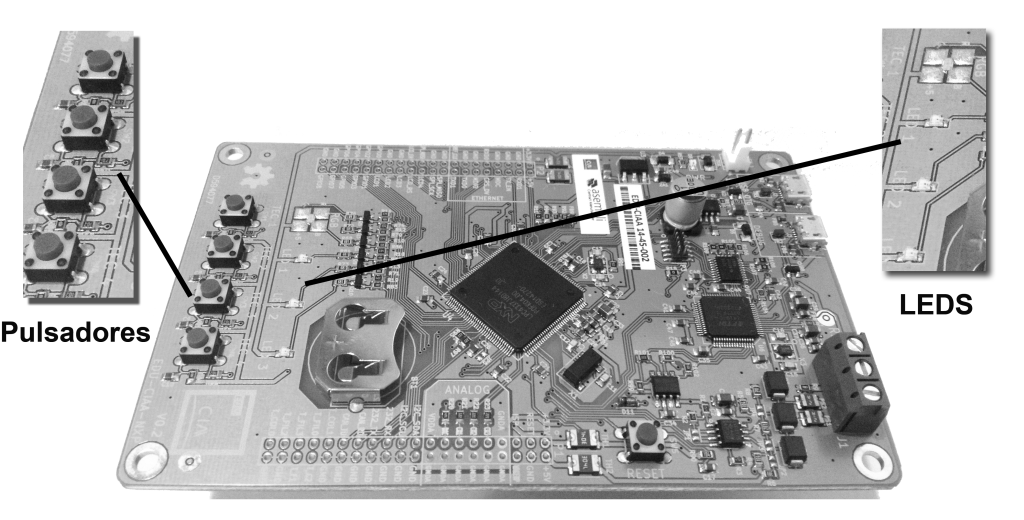
\includegraphics[width=0.7\textwidth]{Figures/fig_educiaa_placa}
  \caption{Foto de una placa EDU-CIAA-NXP}
  \label{fig:educiaaPlaca}
\end{figure}

El diseño fue pensado para proveer una plataforma de desarrollo moderna y económica basada en la CIAA que sirva a docentes y a estudiantes en los cursos de sistemas embebidos y lograr una amplia inserción en el sistema educativo argentino.

En la figura \ref{fig:educiaaPlaca} se muestra una foto de una placa EDU-CIAA-NXP en donde se puede observar claramente los 4 pulsadores y los leds SMD que permiten realizar ejercicios sin requerir componentes adicionales.

%----------------------------------------------------------------------------------------

\section{Utilización de MicroPython}
\label{sec:micropython}

El proyecto MicroPython \cite{micropython} es un desarrollo de firmware realizado por Damien George, el cual fue pensado para correr sobre la plataforma Pyboard, desarrollada por Jaltek Systems \cite{jaltek}. Este proyecto permite la ejecución de código Python y la utilización de los periféricos que posee la placa, desde dicho lenguaje.

\begin{figure}[ht]
  \centering
    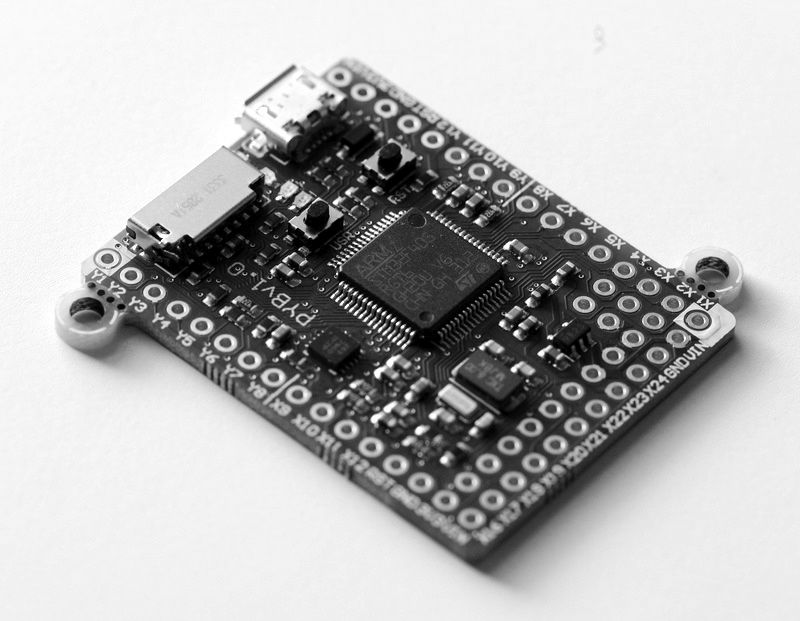
\includegraphics[width=0.4\textwidth]{Figures/fig_pyboard}
  \caption{Foto de una placa Pyboard}
  \label{fig:pyboardPlaca}
\end{figure}

Las características del microcontrolador que posee esta placa, son similares a las de la EDU-CIAA-NXP (Cortex-M4@168Mhz).

Para obtener la capacidad de ejecutar código Python en la EDU-CIAA-NXP, se adoptó el trabajo de Martin Ribelotta, quien realizó el port del proyecto MicroPython mencionado previamente para esta plataforma \cite{portmicropythonribelotta}.
Este port constaba de la inicialización del intérprete, el cual permitía ejecutar código Python, la inicialización y configuración de la \textit{Garbage Collector}\footnote{Garbage Collector: Gestor automático de memoria dinámica.} y la implementación de un filesystem FAT12 embebido en la memoria de programa del microcontrolador, de manera de poder escribir en forma permanente el código Python en la memoria y luego ser ejecutado desde allí. 

%El port no contaba con la implementación para el manejo de los periféricos del microcontrolador, el autor comenzó a desarrollar el soporte para algunos periféricos antes de dar comienzo a este trabajo, dicho soporte se tomó como punto de partida y se reescribió y mejoró en gran medida para lograr la calidad del firmware deseada al implementar técnicas de ingeniería de software.

El autor del presente trabajo comenzó a desarrollar el soporte para algunos periféricos a mediados de 2015, ya que el port de Martin Ribelotta no contaba con la implementación para el manejo de dichos periféricos. Esto se tomó como punto de partida y se reescribió y mejoró en gran medida para lograr la calidad del firmware deseada al implementar técnicas de ingeniería de software.
%----------------------------------------------------------------------------------------

\section{Arquitectura del Firmware}
\label{sec:firmwareArq}

A continuación se detallará la arquitectura del firmware implementado en este trabajo. En la misma se pueden apreciar los siguientes bloques:

\begin{itemize}
	\item \textbf{EDU-CIAA-NXP}: representa el hardware donde se ejecuta el firmware.
	\item \textbf{Intérprete uPython}: representa el código del proyecto MicroPython, mediante el cual es posible interpretar y ejecutar el código Python escrito por el usuario.
	\item \textbf{Código Python programado por el usuario}: representa el código que el usuario escribe en el IDE y graba en la placa para su posterior ejecución.
\end{itemize}

\begin{figure}[ht]
  \centering
    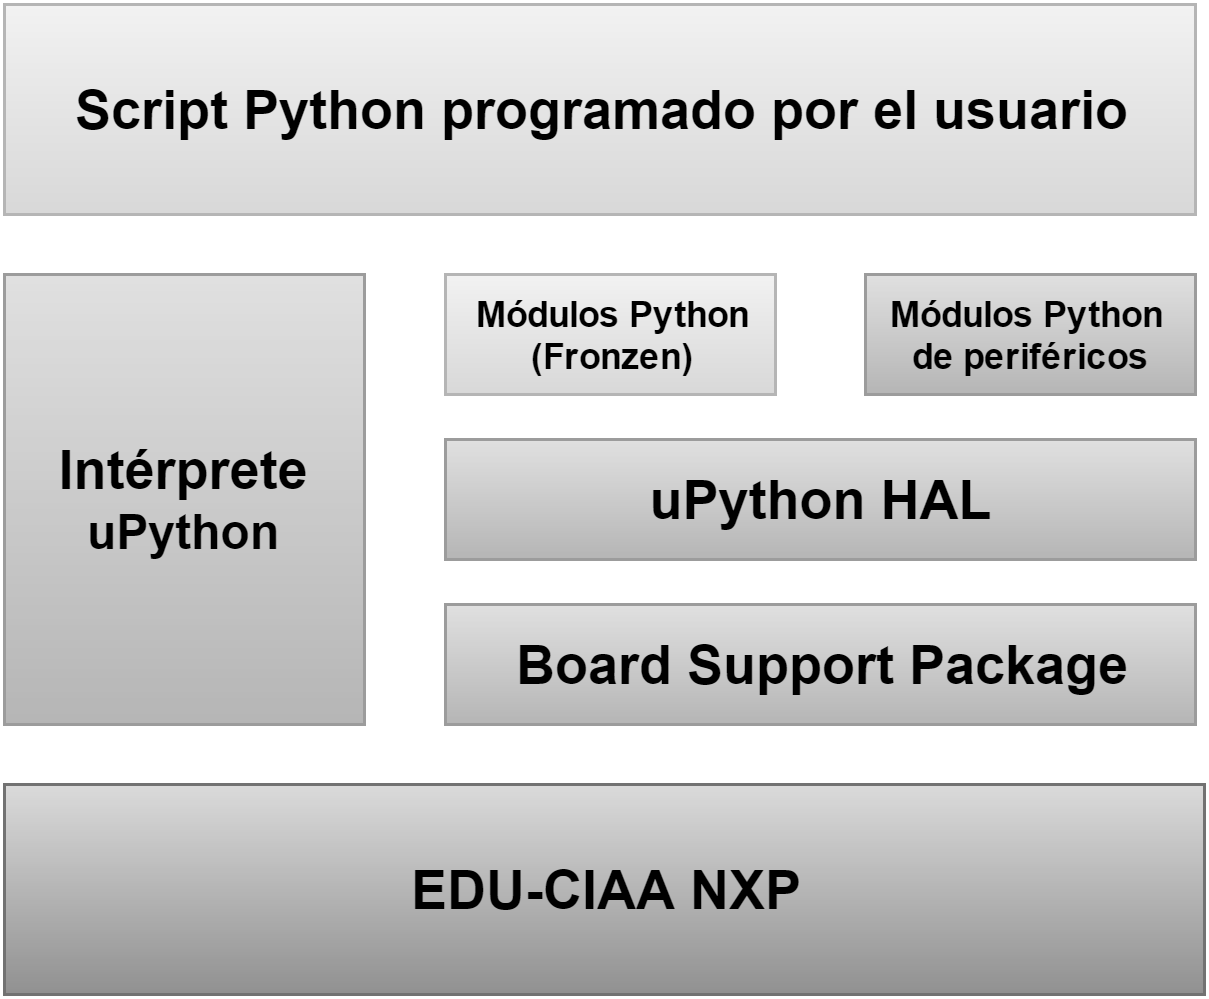
\includegraphics[width=0.7\textwidth]{Figures/fig_firm_arquitectura}
  \caption{Diagrama en bloques de la arquitectura del Firmware}
  \label{fig:firmwareArq}
\end{figure}

Estos tres bloques mencionados y que pueden identificarse en la figura \ref{fig:firmwareArq} representan el firmware del proyecto MicroPython creado por Martin Ribelotta que se tomó como punto de partida para el desarrollo de este trabajo. 

A continuación se detallan los bloques que se han desarrollado:

\begin{itemize}
	\item \textbf{Board Support Package}: aquí se encuentra la biblioteca que permite el acceso, uso e inicialización de los periféricos del microcontrolador.
	\item \textbf{uPython HAL}: capa de abstracción del hardware. El proyecto MicroPython utiliza esta capa para abstraer funciones específicas del hardware y que el código que utilice los periféricos sea portable.
	\item \textbf{Módulos Python de periféricos}: para que el usuario pueda utilizar los periféricos desde el código Python, se necesita escribir un código en lenguaje C que represente una clase Python, en dicho código se consigue ejecutar funciones de C al ejecutar funciones de Python, de esta manera se logra utilizar la capa uPython HAL desde el código Python escrito por el usuario.
	\item \textbf{Módulos Python (Frozen)}: también es posible escribir bibliotecas Python directamente en lenguaje Python, y que las mismas formen parte del firmware. Este trabajo incluyó una biblioteca escrita en Python que permite la ejecución de tests unitarios.
\end{itemize}

%----------------------------------------------------------------------------------------

\section{Arquitectura del Software}
\label{sec:softwareArq}

A continuación se detallará la arquitectura del entorno de desarrollo, en la cual se describe la utilización de una ventana principal en donde se puede editar el archivo de código Python, y mediante un mecanismo de plug-ins se indica la incorporación de ventanas específicas que tienen que ver con el proceso de grabar el código en la EDU-CIAA-NXP. 

\begin{figure}[ht]
  \centering
    \includegraphics[width=0.8\textwidth]{Figures/fig_soft_arquitectura}
  \caption{Diagrama en bloques de la arquitectura del Software del IDE}
  \label{fig:softwareArq}
\end{figure}

En la figura \ref{fig:softwareArq} se observan los siguientes módulos de software que componen el IDE:

\begin{itemize}
	\item \textbf{Archivo .py}: representa el archivo que se abre, edita y guarda usando el IDE. En este archivo se escribirá el código Python que se grabará y ejecutará en la placa.
	\item \textbf{Editor de archivo .py}: representa la capa gráfica del programa en donde se escribe el código Python.
	\item \textbf{Lógica del editor}: representa las funciones que permiten que la ventana principal donde se escribe el código funcione como un editor de texto.
	\item \textbf{Sistema de plug-ins}: la lógica del editor incorpora un sistema de plug-ins mediante el cual se agregan opciones al menú y permiten ejecutar ventanas adicionales a la principal.
	\item \textbf{Menú para la EDU-CIAA-NXP}: aquí se encuentran las opciones que permiten interactuar con la placa y los ejemplos.
\end{itemize}

Dentro de las ventanas agregadas, se encuentran las que permiten la grabación del código en la placa, la ejecución de una terminal serial, mediante la cual es posible visualizar el standard output del código Python e ingresar datos por el standard input, una ventana con una lista de porciones de código de ejemplo (Snippets) y una ventana de configuración en donde se declara el puerto serie de la PC a utilizar.
A continuación se detallan los módulos de software correspondientes a las ventanas mencionadas previamente:

\begin{itemize}
	\item \textbf{Ventana de configuración}: aquí se permite elegir el puerto serie de la PC en donde se conectó la placa.
	\item \textbf{Lógica configuración}: representa las funciones que manejan la ventana de configuración.
	\item \textbf{Ventana de grabación}: aquí se muestra el progreso del envío del archivo a la placa.
	\item \textbf{Lógica de grabación}: representa las funciones que se encargan de enviar el archivo a la placa y mostrar el progreso en la ventana de grabación.
	\item \textbf{Ventana de Snippets}: aquí se muestra una lista de porciones de código de ejemplo y mediante un botón se puede agregar dicha porción de código al archivo que se está escribiendo.
	\item \textbf{Lógica de Snippets}: representa las funciones que manejan la interacción del usuario con la ventana de Snippets.
	\item \textbf{Ventana terminal serie}: aquí se muestra el stdout del código de Python que se ejecuta en la placa y se capturan las teclas que presiona el usuario y se envian hacia el stdin del código Python que se ejecuta en la placa.
	\item \textbf{Lógica terminal serie}: representa las funciones encargadas de la comunicación serie y representación en la ventana.
\end{itemize}
	
El desarrollo de este IDE se basó en el IDE del proyecto EDILE \cite{edile}, y se agregaron las ventanas específicas mencionadas previamente.





%----------------------------------------------------------------------------------------


\section{Requerimientos}
\label{sec:req}

A continuación se detallan los requerimientos planteados para la realización de este trabajo.

Grupo de requerimientos referidos a las bibliotecas Python:
\begin{enumerate}
	\item  Manejo de los leds que dispone la placa.
	\item  Utilización de los pulsadores.
	\item  Manejo y configuración de los pines designados como GPIO. 
	\item  Configuración y utilización de la UART.
	\item  Configuración y utilización de la interface RS485.
	\item  Lectura de las entradas ADC.
	\item  Salida DAC.
	\item  Utilización de la EEPROM interna.
	\item  Utilización de Timers.
\end{enumerate}

Grupo de requerimientos referidos al entorno de desarrollo:
\begin{enumerate}
	\item  El software deberá ser multiplataforma (Windows/Linux/OSX).
	\item  No debe ser necesario recompilar el firmware de la placa para cambiar el código de python.
	\item  El programa de python se enviará por el COM virtual generado al conectar la placa a la PC. 
	\item  El software deberá tener embebida una terminal serial, por donde se implementará la interfaz de salida y entrada estándar del programa de Python. 
	\item  El software deberá tener porciones de código de ejemplo que puedan insertarse fácilmente junto con lo que el usuario programa (Snippets)
	\item  El software deberá tener links para acceder fácilmente a la documentación online y a los proyectos de ejemplo.
\end{enumerate}

Grupo de requerimientos referidos a los proyectos de ejemplo:
\begin{enumerate}
	\item  Los proyectos de ejemplo serán divididos en tres categorías: Inicial, Intermedio y Avanzado. 
	\item  Los proyectos de ejemplo consistirán en el código fuente, la explicación del mismo en forma detallada, y un esquemático de conexión con componentes externos en el caso que se requiera.
	\item  Los proyectos de ejemplo están basados en los proyectos típicos de electrónica que se realizan en escuelas secundarias. 
\end{enumerate}

Grupo de requerimientos generales:
\begin{enumerate}
	\item  El acceso a la información del proyecto será libre y gratuita.  
	\item  Se publicará la documentación de las bibliotecas de Python disponibles para programar.
\end{enumerate}


%----------------------------------------------------------------------------------------


 
\chapter{Diseño e Implementación} % Main chapter title

\label{Chapter3} % Change X to a consecutive number; for referencing this chapter elsewhere, use \ref{ChapterX}
\definecolor{mygreen}{rgb}{0,0.6,0}
\definecolor{mygray}{rgb}{0.5,0.5,0.5}
\definecolor{mymauve}{rgb}{0.58,0,0.82}

\lstset{ %
  backgroundcolor=\color{white},   % choose the background color; you must add \usepackage{color} or \usepackage{xcolor}
  basicstyle=\footnotesize,        % the size of the fonts that are used for the code
  breakatwhitespace=false,         % sets if automatic breaks should only happen at whitespace
  breaklines=true,                 % sets automatic line breaking
  captionpos=b,                    % sets the caption-position to bottom
  commentstyle=\color{mygray},    % comment style
  deletekeywords={...},            % if you want to delete keywords from the given language
  %escapeinside={\%*}{*)},          % if you want to add LaTeX within your code
  %extendedchars=true,              % lets you use non-ASCII characters; for 8-bits encodings only, does not work with UTF-8
  %frame=single,	                   % adds a frame around the code
  keepspaces=true,                 % keeps spaces in text, useful for keeping indentation of code (possibly needs columns=flexible)
  keywordstyle=\bfseries\color{black},       % keyword style
  language=[ANSI]C,					% the language of the code
  %otherkeywords={*,...},           % if you want to add more keywords to the set
  numbers=left,                    % where to put the line-numbers; possible values are (none, left, right)
  numbersep=5pt,                   % how far the line-numbers are from the code
  numberstyle=\tiny\color{mygray}, % the style that is used for the line-numbers
  rulecolor=\color{black},         % if not set, the frame-color may be changed on line-breaks within not-black text (e.g. comments (green here))
  showspaces=false,                % show spaces everywhere adding particular underscores; it overrides 'showstringspaces'
  showstringspaces=false,          % underline spaces within strings only
  showtabs=false,                  % show tabs within strings adding particular underscores
  stepnumber=1,                    % the step between two line-numbers. If it's 1, each line will be numbered
  stringstyle=\bfseries\color{black},     % string literal style
  tabsize=2,	                   % sets default tabsize to 2 spaces
  title=\lstname,                   % show the filename of files included with \lstinputlisting; also try caption instead of title
  morecomment=[s]{/*}{*/}%
}


En este capítulo se detalla el desarrollo del firmware, software y documentación.

%----------------------------------------------------------------------------------------
%	SECTION 1 : Diseño de Firmware
%----------------------------------------------------------------------------------------
\section{Diseño del Firmware}

\subsection{Punto de partida} 

Al tomar el port de MicroPython para la EDU-CIAA-NXP desarrollado por Martín Ribelotta, era posible ejecutar un intérprete \textit{REPL}\footnote{REPL: Read Eval Print Loop. Mecanismo que toma una expresión escrita por el usuario, la evalúa y ejecuta, devolviendo el resultado al usuario.} que provee el proyecto, el cual tiene como standard input (stdin) y standard output (stdout) el puerto serie que la placa tiene conectado a través del conversor USB, de modo que en la PC se crea un COM Virtual que permite a cualquier programa que emula una terminal por puerto serial, conectarse a dicho intérprete.

En la figura \ref{fig:conexion} se observan los bloques que modelan la conexión de la placa con la PC. Mediante el circuito integrado FT2232 que posee la placa, se conecta por medio del bus USB, la PC a la EDU-CIAA-NXP, permitiendo visualizar uno de los módulos UART del microcontrolador como un puerto serie en la PC.

\begin{figure}[h]
  \centering
    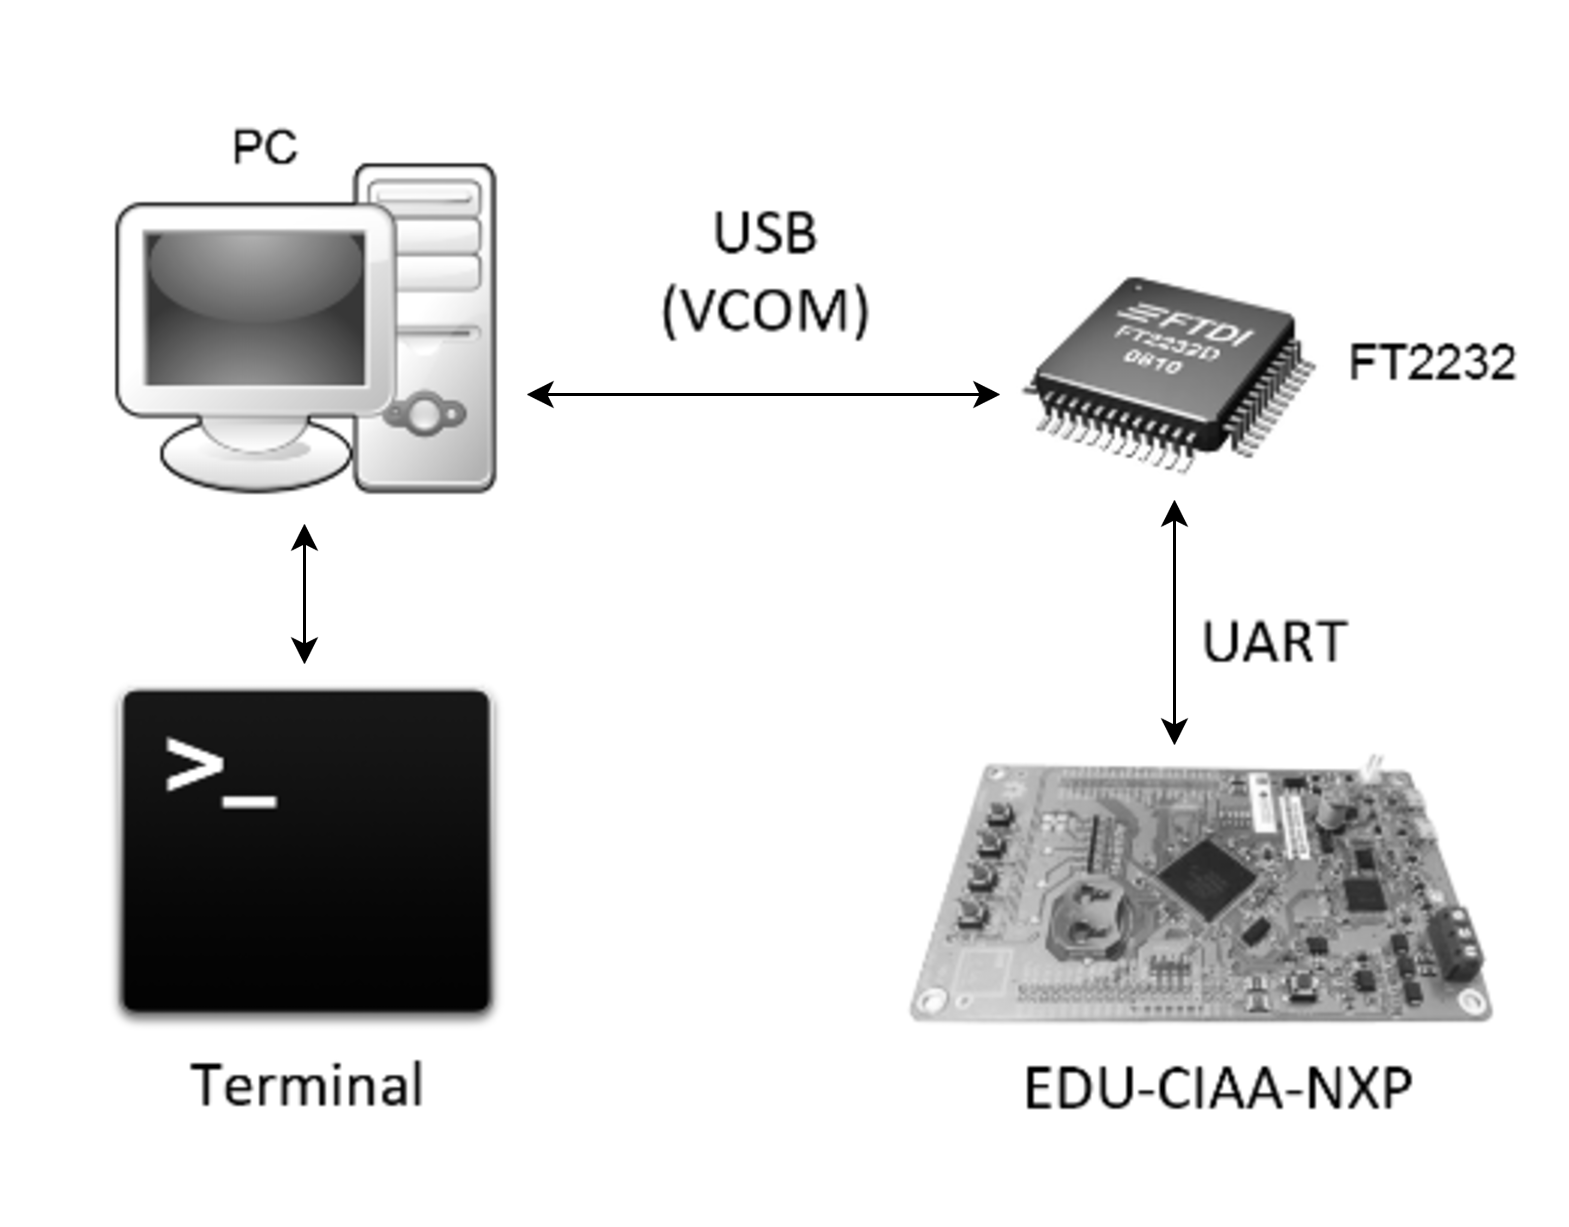
\includegraphics[width=0.7\textwidth]{Figures/fig_conexion}
  \caption{Conexión de la EDU-CIAA-NXP con la PC}
  \label{fig:conexion}
\end{figure}

Esto permite ejecutar programas que no tengan interacción con el resto del hardware, por ejemplo, se puede escribir:

\textbf{{\fontsize{16}{16}\selectfont \textgreater\textgreater}} \texttt{print(“Hola mundo”)}

Una vez ingresado el código, el interprete lo evalúa y ejecuta, y el texto “Hola mundo” se transmite por el stdout, el cual está ligado a la UART conectada al conversor serie-USB, por lo que el texto “Hola mundo” se muestra por la terminal de la PC.

De la misma forma se puede utilizar el sdtin con sentencias como:

\textbf{{\fontsize{16}{16}\selectfont \textgreater\textgreater}} \texttt{n = input(“Ingrese un numero”)}

También se pueden realizar operaciones matemáticas como por ejemplo:

\textbf{{\fontsize{16}{16}\selectfont \textgreater\textgreater}} \texttt{a = 27}\\
\textbf{{\fontsize{16}{16}\selectfont \textgreater\textgreater}} \texttt{b = 3}\\
\textbf{{\fontsize{16}{16}\selectfont \textgreater\textgreater}} \texttt{c = a + b}\\
\textbf{{\fontsize{16}{16}\selectfont \textgreater\textgreater}} \texttt{print(c)}

Este último ejemplo imprime por la terminal el valor 30.

Pero para interactuar con los periféricos como los pulsadores y los leds, solo existía una versión preliminar de algunas bibliotecas Python creadas previamente por el autor de este trabajo, las cuales se tomaron como punto de partida para el desarrollo profesional de las mismas verificando su correcto funcionamiento por medio de test unitarios y funcionales los cuales son explicados en el capítulo \ref{Chapter4}.

%----------------------------------------------------------------------------------------

\subsection{Creación de bibliotecas Python: Módulos y Clases} 

Si bien es posible definir funciones sueltas sin contexto, en Python también es posible la declaración de clases, al ser un lenguaje multiparadigma, el mismo contempla la Programación Orientada a Objetos (POO), mediante la cual se modelaron los periféricos del microcontrolador.

En Python, las clases se agrupan dentro de módulos. Un módulo Python es un conjunto de clases, para poder utilizar una clase que se encuentra dentro de un módulo, deberemos incluir dicho módulo en nuestro programa, mediante la sentencia import, por ejemplo:

\textbf{{\fontsize{16}{16}\selectfont \textgreater\textgreater}} \texttt{import pyb}

El módulo pyb tiene dentro definidas las clases que representan los periféricos del microcontrolador. Una vez incluído el módulo, podremos utilizar las clases definidas dentro de él para crear objetos.
Por ejemplo, para la creación de un objeto que representa el led 1 de la EDU-CIAA-NXP, se escribe:

\textbf{{\fontsize{16}{16}\selectfont \textgreater\textgreater}} \texttt{import pyb}\\
\textbf{{\fontsize{16}{16}\selectfont \textgreater\textgreater}} \texttt{led = pyb.LED(1)}\\
\textbf{{\fontsize{16}{16}\selectfont \textgreater\textgreater}} \texttt{led.on()}

En este ejemplo se utiliza la clase LED para crear el objeto led, la misma recibe como argumento de su constructor, el número de led que el objeto manejará, en este caso, el led 1.

Para poder manejar un periférico del microcontrolador (GPIOs, UART, etc.) es necesario que al ejecutar una o más funciones de código Python, se ejecute una o más funciones de código C, en la cual se coloca el código necesario para la utilización del periférico en cuestión.

En la figura \ref{fig:calls} se muestra un diagrama donde se aprecia el \textit{trace}\footnote{Tracing: Log que muestra información acerca de la ejecución de un programa junto con las llamadas a funciones.} de las llamadas a función que se ejecutan cuando el usuario ejecuta desde código Python el método on() de un objeto LED.

\begin{figure}[ht]
  \centering
    \includegraphics[width=1.05\textwidth]{Figures/fig_calls}
  \caption{Anidamiento de llamadas a funciones desde Python a C}
  \label{fig:calls}
\end{figure}

Al ejecutarse la llamada del método on() desde el objeto led, se produce la ejecución de la función pyb\_led\_on() la cual se encuentra definida en el archivo modpybled.c, en este archivo están declaradas todas las funciones que se mapean a métodos del objeto LED. Cada método que pose el objeto led tendrá asociada una función dentro del archivo modpybled.c.

Estos archivos modpybXXX.c representan la clase de un periférico (en este ejemplo modpybled.c representa la clase LED) y utilizan las funciones de la capa de abstracción de hardware (uPython HAL) definidas en ciaanxp\_mphal.c para acceder y utilizar los periféricos.
Dentro de la capa uPython HAL, se utilizan las funciones definidas en la capa Board Support Package (archivo board.c) en donde se utilizan las funciones de la biblioteca \textit{LPCOpen}\footnote{LPCOpen: Biblioteca desarrollada por NXP la cual provee macros y funciones para acceder a los registros del microcontrolador desde lenguaje C.} para el manejo de periféricos.

En la figura \ref{fig:files} se observan los archivos implicados para poder brindar desde el código Python una interfaz para el uso de cada periférico. En ella se observa que existe un archivo modpybXXX.c para definir cada clase Python. Dentro de cada archivo se definen las funciones de C que se ejecutarán al invocar los métodos desde Python. Estas funciones de C utilizan la capa uPython HAL para interactuar con los periféricos del microcontrolador.
Para una explicación detallada sobre el desarrollo de una clase Python desde código C, referirse al apéndice \ref{AppendixA}

\begin{figure}[ht]
  \centering
    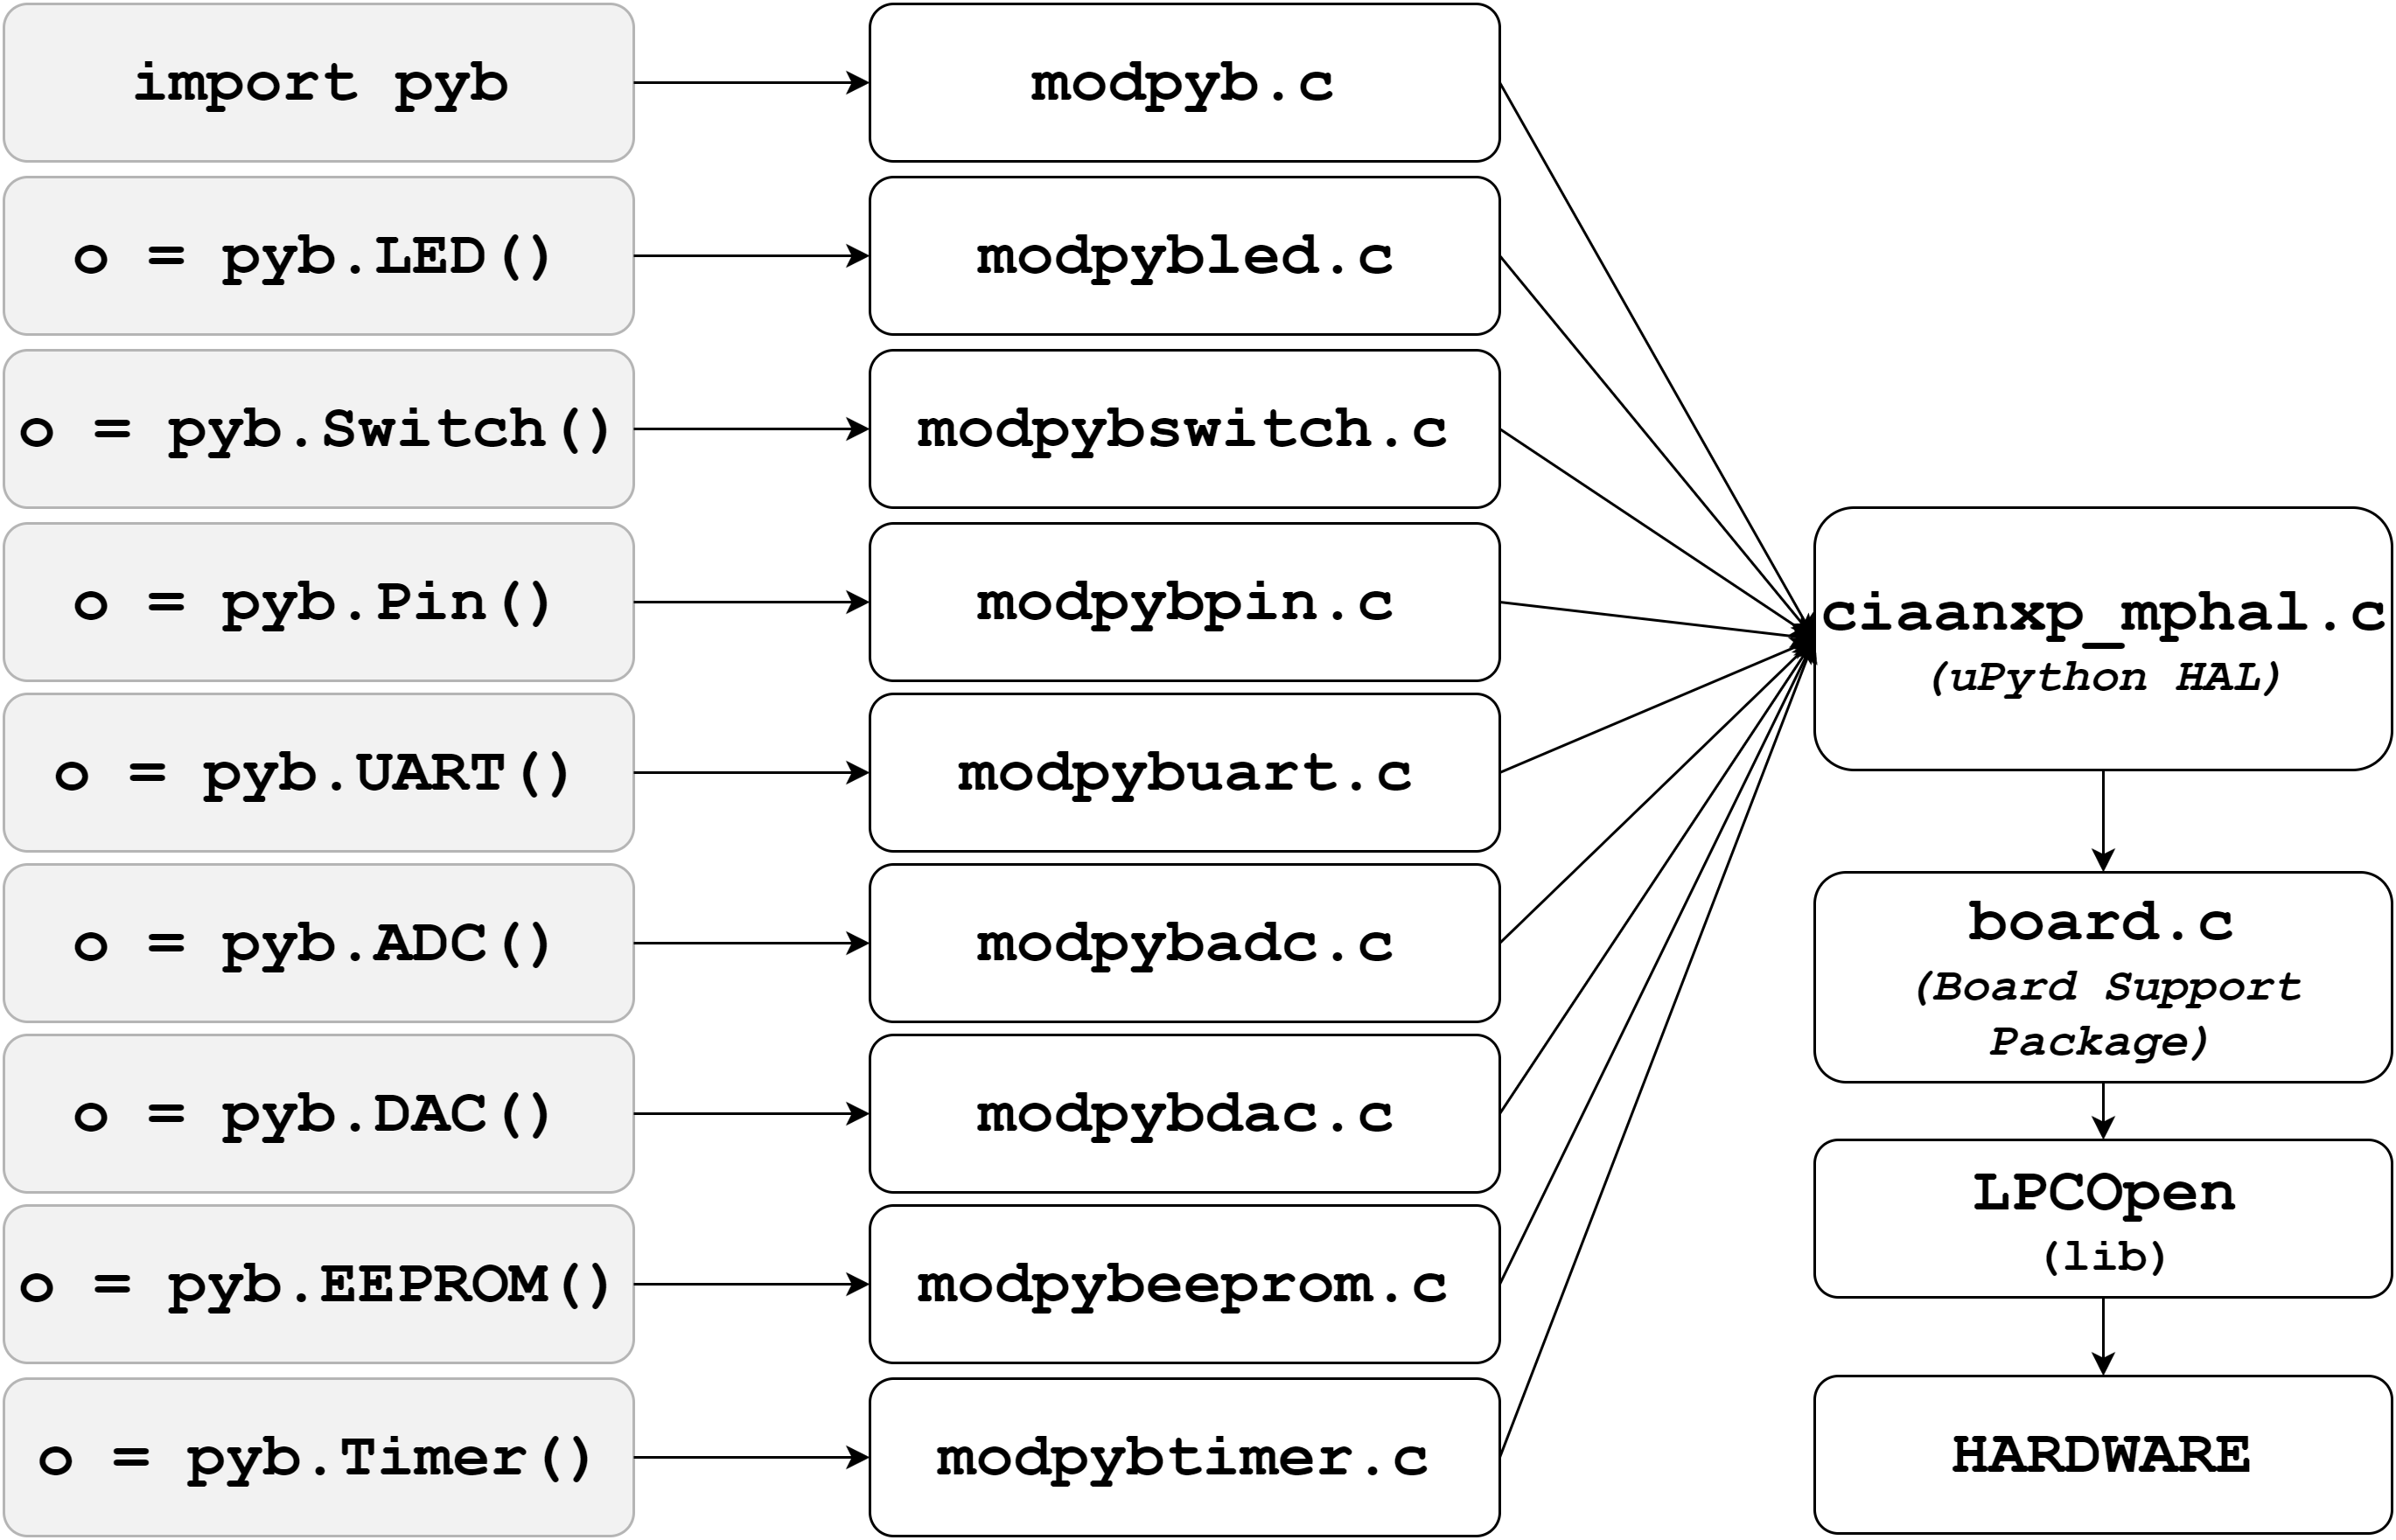
\includegraphics[width=0.95\textwidth]{Figures/fig_files}
  \caption{Relación entre las clases Python y los archivos del firmware}
  \label{fig:files}
\end{figure}

%----------------------------------------------------------------------------------------

\subsection{Diseño de bibliotecas para el manejo de periféricos desde C}

En el archivo board.c y board.h se definió la capa Board Support Package (BSP), mediante la cual se accede a los periféricos del microcontrolador, en este archivo se definieron las funciones para inicializar y utilizar dichos periféricos, requiriendo la menor cantidad de datos de inicialización posibles y abstrayendo en gran medida la arquitectura del microprocesador.

Esta capa utiliza la biblioteca LPCOpen, la cual es de más bajo nivel pero permite un fácil acceso a los registros del microcontrolador, proveyendo funciones y macros para resolver este problema.

Las funciones definidas en board.c tienen el formato:

\begin{verbatim}
Board_NombrePeriferico_NombreFuncion()
\end{verbatim}

Algunos ejemplos de las funciones que pueden encontrarse en este archivo son:

\begin{verbatim}
void Board_LED_Set(uint8_t LEDNumber, bool On);
bool Board_LED_Test(uint8_t LEDNumber);
void Board_LED_Toggle(uint8_t LEDNumber);
\end{verbatim}

Todos los periféricos tienen su función Init:
\begin{verbatim}
Board_NombrePeriferico_Init()
\end{verbatim}

la cual se encarga de inicializar dicho periférico. Existe también en el archivo, definida una función principal que se encarga de llamar a todas las funciones “Init” y es llamada “Board\_Init()”

Como se indica en la figura \ref{fig:calls}, las funciones definidas en esta capa son ejecutadas por las funciones definidas en la capa uPython HAL, las cuales se definen en el archivo ciaanxp\_mphal.c y ciaanxp\_mphal.h.

La capa uPython HAL, es prácticamente transparente, ya que en la mayoría de los casos no agrega funcionalidades, y simplemente invoca a las funciones de la capa BSP. 
Sin embargo en algunos casos en donde las funciones definidas en BSP no cubren las características necesarias para ser utilizadas desde Python, se han agregado las características en esta capa.

También se han agregado porciones de código para validación de rangos o para agregar argumentos, como se muestra en el algoritmo \ref{lst:uarthal} en donde se define la función para enviar por el puerto serie.

\begin{lstlisting}[label={lst:uarthal},caption=Función de envío por la UART de la capa uPython HAL] 
uint32_t mp_hal_rs232_write(uint8_t const * const buffer, 
                                     uint32_t size,uint32_t delay)
{
    if(delay==0)
        return Board_UART_Write(LPC_USART3,buffer,size);

    uint32_t i=0;
    while(size>0)
    {
        Board_UART_Write(LPC_USART3,&(buffer[i]),1);
        mp_hal_milli_delay(delay);
        size--;
        i++;
    }
    return i;
}
\end{lstlisting}

En este caso se observa que la función de la capa uPython HAL tiene un argumento que indica un retardo (delay) entre cada byte que se envía (línea 2), funcionalidad que no existe en la capa BSP, ya que solo se dispone de la función “Board\_UART\_Write()” la cual recibe el buffer a transmitir.
En esta función se evalúa el valor del argumento delay, y en el caso de que sea mayor a cero, se harán envíos de 1 byte y por cada envío se ejecutará la función “mp\_hal\_milli\_delay()” la cual boquea el código por el tiempo especificado.

Las funciones de la capa uPython HAL tienen la forma:

\begin{verbatim}
mp_hal_nombrePeriferico_nombreFuncion()
\end{verbatim}

Tanto la biblioteca BSP como la capa uPython HAL pueden utilizarse de forma aislada en un proyecto \textit{baremetal}\footnote{Baremetal: Método de programación de bajo nivel para un hardware específico utilizando herramientas básicas y sin un sistema operativo.} para el microcontrolador LPC4337, proveyendo un acceso simple a los periféricos del mismo.

%----------------------------------------------------------------------------------------

\subsection{Diseño de bibliotecas para el manejo de periféricos desde el código Python}

Se pretendió modelar cada periférico mediante una clase, si bien era posible definir funciones pertenecientes al módulo pyb, sin definir clases, por ejemplo:

\textbf{{\fontsize{16}{16}\selectfont \textgreater\textgreater}} \texttt{pyb.setLed(1,0)}

Se decidió respetar el modelo orientado a objetos por las siguientes razones:

\begin{itemize}
	\item El proyecto MicroPython original utiliza este modelo para acceder a los periféricos.
	\item Ayuda al entendimiento de programación orientada a objetos (POO), en donde la premisa más básica es representar objetos del mundo real, en este caso un objeto Switch representará un pulsador físico en la placa, generando un ejemplo muy claro del concepto.
	\item Para el uso básico y explicaciones de algoritmo, no es necesario tener los conocimientos de POO, simplemente se trata al objeto como una variable, y no se generan grandes trabas en el momento del aprendizaje.
\end{itemize}

En la figura \ref{fig:classes} se observa el diagrama de clases definido para el módulo pyb, en donde se encuentran las clases que representan los periféricos del microcontrolador junto con los métodos desarrollados.

\begin{figure}[ht]
  \centering
    \includegraphics[width=1.1\textwidth]{Figures/fig_classes_diagram}
  \caption{Diagrama de clases para manejo de periféricos}
  \label{fig:classes}
\end{figure}

%----------------------------------------------------------------------------------------
%	SECTION 2: Diseño del Software
%----------------------------------------------------------------------------------------
\section{Diseño del Software}

\subsection{Punto de partida} 

Para el desarrollo del IDE se tomó como base el proyecto EDILE \cite{edile} el cual se muestra en la figura \ref{fig:edile}. El mismo se encuentra escrito en lenguaje Python y proporciona un procesador de texto con coloreado de palabras clave según el lenguaje seleccionado, el cual se detecta automáticamente por la extensión del archivo que se abre.

\begin{figure}[ht]
  \centering
    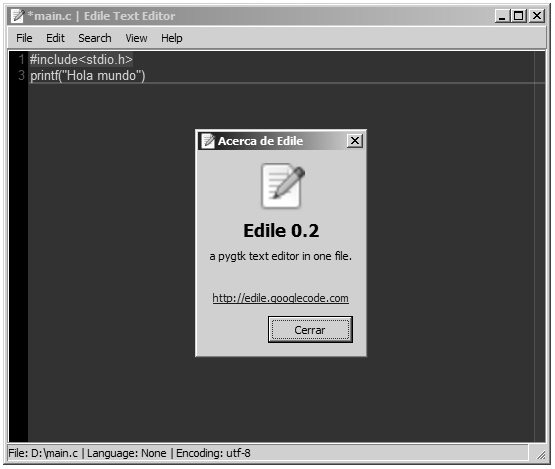
\includegraphics[width=0.7\textwidth]{Figures/fig_edile}
  \caption{Procesador de texto EDILE v0.2}
  \label{fig:edile}
\end{figure}

Debido a que se encuentra programado en Python es muy simple ejecutar el programa en diferentes sistemas operativos, de modo que utilizando este proyecto se puede cumplir con uno de los requerimientos planteados el cual decía que el software debe ser multiplataforma.

Este procesador de texto posee un sistema de plug-ins mediante el cual se simplifica la incorporación de menúes que ejecuten ventanas adicionales que cumplan con cierta funcionalidad, de modo que el diseño de software que se realizó en el presente trabajo fue la incorporación de dichas ventanas y funcionalidades al editor, junto con modificaciones para que solo trabaje con archivos de código Python (.py) y algunas correcciones en el sistema de plug-ins.

Junto con las modificaciones mencionadas, se escribieron test unitarios para las ventanas y clases de lógica desarrolladas, asegurando al igual que en el firmware, la calidad del software requerida para un trabajo de especialización.

\subsection{Diseño del IDE} 

Se modificó el código del proyecto EDILE y se incorporó una barra de botones junto con una nueva opción de menú, llamada “EDU-CIAA”. La incorporación de este nuevo menú fue posible gracias al sistema de plug-ins con el que cuenta en editor base, en la figura \ref{fig:idebuttons} se aprecia el menú agregado así como también los botones que poseen las mismas funcionalidades que las opciones del menú.

\begin{figure}[ht]
  \centering
    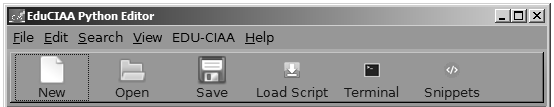
\includegraphics[width=0.7\textwidth]{Figures/fig_ide_buttons}
  \caption{Botones adicionales del IDE.}
  \label{fig:idebuttons}
\end{figure}

En la figura \ref{fig:ideclasses} se observan las clases desarrolladas. La clase que funciona como un plug-in del editor, es la llamada mnu\_EDUCIAA, en ella se ejecutan métodos según qué opción de menú eligió el usuario (o qué botón presionó). Esta clase hace las veces de \textit{controller}\footnote{controller: Componente del patrón de diseño MVC el cual se encarga de recibir eventos y realizar acciones.} y dispara las diferentes ventanas según la opción seleccionada.

\begin{figure}[ht]
  \centering
    \includegraphics[width=0.99\textwidth]{Figures/fig_ide_classes}
  \caption{Diagrama de clases de las funcionalidades agregadas al IDE.}
  \label{fig:ideclasses}
\end{figure}

 A continuación se detallan las clases creadas:

\begin{itemize}
	\item \textbf{mnu\_EDUCIAA}: recibe los eventos de click sobre los ítems del menú o los botones y lanza las diferentes ventanas (Terminal serie, Configuración, Snippets y Grabación).
	\item \textbf{Console}: ventana que se conecta por el puerto serial configurado y muestra en pantalla los caracteres recibidos, de la misma forma captura las teclas que el usuario presiona y las envía.
	\item \textbf{ConfigWindow}: ventana que permite al usuario configurar el puerto serie mediante el cual se comunica el IDE con la EDU-CIAA-NXP.
	\item \textbf{SnippetsWindow}: ventana que muestra una lista de porciones de código de ejemplo, y que por medio de un botón permite agregarlas al texto que el usuario está escribiendo.
	\item \textbf{LoadScriptWindow}: ventana que se encarga del envío del archivo a la placa utilizando el protocolo xmodem y de mostrar el progreso.
	\item \textbf{ConfigManager}: esta clase se encarga de escribir y leer en un archivo la configuración del IDE (es decir el puerto serie que seleccionó el usuario).
	\item \textbf{SnippetsParser}: todos los ejemplos que se muestran en la ventana de Snippets, se leen de un archivo XML. Esta clase se encarga de leer dicho archivo y devolver la información para que la ventana la pueda mostrar.	
	\item \textbf{Protocol}: recibe como dato el puerto serie y la ruta al archivo a transmitir, y se encarga de utilizar la biblioteca XMODEM para enviar el archivo hacia la placa.
	\item \textbf{XMODEM}: biblioteca que implementa el protocolo \textit{xmodem}\footnote{xmodem: Protocolo simple de transferencia de datos por medio de paquetes de 128bytes creado en 1977.} y permite el envío del archivo a la placa.	
\end{itemize}

El diseño de las ventanas y sus contenidos fueron creados con el programa Glade \cite{glade} utilizado para crear ventanas para la biblioteca gráfica pyGTK.

La lógica de cada ventana se encuentra implementada dentro de cada una de las clases, las cuales utilizan la biblioteca pyGTK para construir la interfaz gráfica por medio de un archivo XML (extensión .glade) donde se define el formato de la ventana y los componentes que posee dentro (Botones, etc.)

En el algoritmo \ref{lst:pygtkbuilder} se muestra la creación del objeto builder el cual obtiene los datos de la ventana gráfica del archivo LoadScriptWindow.glade, archivo creado con el programa Glade. Luego en la línea 8 se observa cómo mediante el método get\_objet() se obtiene una referencia de un objeto Button definido para dicha ventana y que tiene asignado el nombre “btnClose”. De esta manera se obtienen las referencias de los objetos definidos en el archivo XML y que componen la ventana, permitiendo la interacción con los mismos desde el código.

\begin{lstlisting}[language={python},label={lst:pygtkbuilder},caption=Porción de código que muestra la creación de la ventana a partir del archivo glade] 
		try:
			builder = gtk.Builder()
			builder.add_from_file(basePath+"/LoadScriptWindow.glade")
		except Exception,e:
			print(e)
			return

		self.buttonClose = builder.get_object("btnClose")
		
\end{lstlisting}

\subsection{Envío del archivo a la placa}

Para el envío del archivo a la placa, se utilizó el protocolo xmodem debido a su sencillez, este protocolo permite la trasferencia de datos en paquetes de 128 bytes o 1kbytes, por cada paquete transferido el receptor envía un acuse de recibo (ACK) o un aviso de que hubo un error (NACK).

En la figura \ref{fig:secuencexmodem} se observa el diagrama de secuencia correspondiente a la transferencia de datos entre el firmware desarrollado y la lógica de la ventana LoadScriptWindow.
En él se observa que al reiniciar la placa mediante su pulsador de reset, el firmware envía una trama NACK por el puerto serie, en el caso de que el IDE se encuentre en el modo de inicializar una grabación (porque el usuario abrió la ventana de grabación) se recibirá dicha trama y se reponderá con el primer paquete de datos de 128bytes, al cual el firmware que recibe dicha trama responderá con ACK si pudo grabarlo en la memoria de programa del microcontrolador o NACK en caso de error. 

\begin{figure}[ht]
  \centering
    \includegraphics[width=0.6\textwidth]{Figures/fig_ide_xmodem}
  \caption{Diagrama de secuencia que describe la comunicación entre el IDE y el firmware.}
  \label{fig:secuencexmodem}
\end{figure}

Este proceso continúa hasta que el IDE envía todas las tramas que corresponden al contenido del archivo que se esta enviando.
El firmware irá agregando los datos recibidos al final de la memoria donde se grabaron los datos de la trama anterior.



%----------------------------------------------------------------------------------------
%	SECTION 3: Documentacion
%----------------------------------------------------------------------------------------
\section{Documentación}

Como se indicó en el capítulo \ref{Chapter1}, el desarrollo del firmware y del software no es suficiente para que un proyecto educativo tenga el impacto deseado, sino que debe estar acompañado por la documentación y los ejemplos adecuados. Esta es la razón por la que el IDE posee una ventana de Snippets con porciones de código de ejemplo, sin embargo esto no es suficiente, ya que no existe explicación alguna de dichas porciones de código. 
Además de los Snippets, se agregaron proyectos de ejemplo y documentación de las clases y métodos desarrollados para el manejo de los periféricos.

\subsection{Proyectos de ejemplo} 

Para la publicación de ejemplos completos, se creó un repositorio público en GitHub \cite{repoejemplos} en donde pueden descargarse diferentes tipos de proyectos con una explicación detallada del código que se implementó. Los ejemplos se dividen en tres categorías:

\begin{itemize}
	\item \textbf{Inicial}: cubren conceptos básicos de programación y del lenguaje Python.
	\item \textbf{Intermedio}: proyectos que requieren conocimientos intermedios de programación y básicos de electrónica.
	\item \textbf{Avanzado}: proyectos que requieren conocimientos avanzados de programación y electrónica..	
\end{itemize}

Cada proyecto es acompañado por un archivo README.md en donde se aclaran las funciones y sentencias utilizadas, y se explica el funcionamiento del código paso por paso.

La idea es que la comunidad que utilice esta plataforma para desarrollar trabajos, en escuelas secundarias o universidades, aporte los trabajos implementados al repositorio, para que otros estudiantes puedan tomarlos como base para nuevos proyectos o simplemente para aprender de lo desarrollado.

\subsection{Documentación de las bibliotecas implementadas} 

Para acompañar a los proyectos de ejemplo y dar una base sólida del uso y soporte de los periféricos, se escribió una documentación detallada de cada clase con todos sus métodos, escribiendo también uno o más ejemplos del uso de algunos métodos en particular.

Esta documentación se escribió en la página del proyecto CIAA, en la sección Python \cite{bibpython}, la cual también es de acceso público, cumpliendo así con uno de los requerimientos mencionados en el capítulo \ref{Chapter2}. El link a esta página se encuentra accesible desde la ventana de Snippets del IDE.








% Chapter Template

\chapter{Ensayos y Resultados} % Main chapter title
En este capítulo se explica el desarrollo e implementación de tests unitarios y funcionales para el firmware y el software.

\label{Chapter4} % Change X to a consecutive number; for referencing this chapter elsewhere, use \ref{ChapterX}

%----------------------------------------------------------------------------------------
%	SECTION 1
%----------------------------------------------------------------------------------------

\section{Tests unitarios para bibliotecas para el manejo de periféricos desde C}
\label{sec:testUnitariosC}

Para asegurar el correcto funcionamiento de las bibliotecas para el manejo de periféricos, se implementaron tests unitarios para la capa uPython HAL utilizando la técnica \textit{TAD}\footnote{TAD:Test-After Development. Técnica en la cual los tests se escriben luego de escribir el código.}. Mediante estos tests se probó el uso de las funciones de dicha capa cubriendo la complejidad ciclomática de cada una de ellas.

Teniendo como principal objetivo un consumo reducido de memoria de datos y de programa para la implementación de los tests (debido a que se ejecutan en la propia placa sin utilizar \textit{mocks}\footnote{Mock:Porción de código simple que simula otra porción de código más compleja.}), no se utilizó ninguna biblioteca existente, sino que se desarrolló una pequeña biblioteca mayormente compuesta por \textit{macros}\footnote{Macro:Fragmento de código con un nombre asociado.El precompilador reemplaza el nombre por el código.}, que permitió ejecutar los tests unitarios de una manera simple y controlada.

En el algotimo \ref{lst:utest} se muestra la función utest\_startTest la cual se encarga de ejecutar un test unitario. La misma recibe los argumentos que se detallan a continuación:

\begin{itemize}
	\item \textbf{fncTest}: una función donde se escribirá el test unitario.
	\item \textbf{fncBefore}: una función que en el caso de existir, se ejecutará antes de fncTest (puede utilizarse para inicializaciones antes de la ejecución del test).
	\item \textbf{testName}: un texto con el nombre del test, el cual se imprime antes de ejecutar las funciones (línea 8).	
\end{itemize}
	
El control de errores se observa en la línea 7 en donde se pone a cero la variable global utest\_flagTestError, luego de la ejecución de las funciones pasadas como argumento, en la línea 13 se evalúa el estado de dicha variable, la cual se pudo cargar con el valor 1 en la función del test si hubo un error. En dicho caso se imprime un mensaje de error (línea 15) indicando mediante otras variables globales el nombre del archivo y el número de línea donde se produjo el error en el test.

\begin{lstlisting}[label={lst:utest},caption=Función que ejecuta un test unitario incluida en el archivo utest.c del firmware.]
void utest_startTest(void(*fncTest)(void),
                     void(*fncBefore)(void),
                     char* testName)
{
	if(fncTest!=0)
	{
		utest_flagTestError=0;
		utest_print1("TESTING:%s\r\n",testName);
		if(fncBefore!=0)
			fncBefore();
		utest_totalTestsCounter++;
		fncTest();
		if(utest_flagTestError==1)
		{
			utest_print2("TEST FAILED. FILE:%s LINE:%d\r\n",
			              utest_fileTestError,utest_lineTestError);
		}
		else
		{
			utest_okTestsCounter++;
		}
	}
} 
\end{lstlisting}

Las variables globales mencionadas previamente se cargan en la ejecución de la función de test, para ello en el archivo utest.h del firmware, se definieron una serie de macros que permiten ejecutar las comparaciones de valores (asserts) del test unitario.

En el algoritmo \ref{lst:utestmacro} se observa una de las macros definidas la cual es utilizada para comparar dos números enteros. En la línea 4 se realiza la comparación de los valores y en el caso de que no sean iguales se imprime un mensaje de error (línea 6) y se cargan las variables globales que son analizadas en la función utest\_startTest.

\begin{lstlisting}[label={lst:utestmacro},caption=Ejemplo de una macro assert incluida en el archivo utest.h del firmware.]

#define utest_assertEqualsInt(A,B)	
{ 
	if(A!=B)
	{ 
		utest_print2("assert equals failed '%d' != '%d'\r\n",A,B); 
		utest_flagTestError=1; 
		utest_lineTestError = __LINE__;  
		utest_fileTestError = __FILE__;
		return; 
	} 
}
\end{lstlisting}

En el algoritmo \ref{lst:testeeprom} puede apreciarse el uso de la macro utest\_assertEqualsInt la cual recibe el valor esperado (-1) y el valor devuelto por la función de la capa uPython HAL que escribe en la EEPROM. Esta función es uno de los tests unitarios escritos para el manejo de la EEPROM del microcontrolador. La macro realiza la comparación, y en caso de error, imprime el mensaje y carga las variables globales necesarias para que se puedan imprimir los datos del error. La sentencia return hace que se termine la ejecución de la función del test.

\begin{lstlisting}[label={lst:testeeprom},caption=Ejemplo de un test unitario para la EEPROM usando una dirección inválida.]
void testEEPROM2(void)
{
	int32_t r = mp_hal_writeByteEEPROM(0x8000,0x55); // invalid address
	utest_assertEqualsInt(-1,(int)r);
}
\end{lstlisting}

Para ejecutar la función testEEPROM2 así como el resto de las funciones de test para todos los periféricos, se definió el archivo mainTest.c, en el cual se ejecutan las llamadas a la función utest\_startTest mencionada en el algoritmo \ref{lst:utest} y en donde se colocaron líneas de código como la que se observa en el algoritmo \ref{lst:testmain} en una función llamada startTesting. 

\begin{lstlisting}[label={lst:testmain},caption=Ejemplo de ejecución de funciones de test en archivo mainTest.c.]
	utest_startTest(testEEPROM1,0,"EEPROM: write/read byte Test");
	utest_startTest(testEEPROM2,0,"EEPROM: write invalid address Test");
	utest_startTest(testEEPROM3,0,"EEPROM: read invalid address Test");
\end{lstlisting}

Esta función startTesting se ejecuta en el main principal del firmware en el caso de que se compile indicando que se quieren ejecutar los tests (ver sección \ref{sec:testUnitariosPlaca}).

La estructura de archivos referidos a los tests se muestra en la figura \ref{fig:utestcarq}. Los archivos llamados testsXXX.c poseen las funciones de cada test unitario referido a cada periferico, las cuales utilizan las macros definidas en utest.h para realizar las comparaciones (asserts). Todos estos archivos se encuentran dentro de una carpeta llamada testing, y los mismos no se incluyen en el firmware excepto que se compile el mismo para ejecutar los tests.

\begin{figure}[ht]
  \centering
    \includegraphics[width=0.7\textwidth]{Figures/fig_utests_c}
  \caption{Estructura de archivos para la ejecución de tests unitarios de la capa uPython HAL.}
  \label{fig:utestcarq}
\end{figure}

%----------------------------------------------------------------------------------------------------------------------------------------------------

\section{Test unitarios para bibliotecas para el manejo de periféricos desde Python}
\label{sec:testUnitariosPython}

Para asegurar el correcto funcionamiento de las bibliotecas para el manejo de periféricos desde Python, se implementaron tests unitarios para todas las clases Python desarrolladas. Mediante estos tests se pretendió probar el uso de los metodos de dicha capa cubriendo la complejidad ciclomática de cada una de ellos.

Una vez más teniendo como principal objetivo un consumo reducido de memoria de datos y de programa para la implementación de los tests, no se utilizó ninguna biblioteca de tests unitarios para Python, sino que se escribió una que posea lo mínimo indispensable para la ejecución de los tests, en un módulo llamado unittest. 

Este módulo forma parte de las bibliotecas Python que pueden escribirse directamente en Python y no en C (bloque Frozen, ver sección \ref{sec:firmwareArq}), e incorporarse al firmware y al conjunto de módulos que el usuario puede utilizar para programar Python.

En esta biblioteca se definió la clase TestCase, una parte de ella puede observarse en el algoritmo \ref{lst:testcase} en donde se muestra la definición de la clase y de los métodos:

\begin{itemize}
	\item \textbf{setUp}: método que se ejecutará antes del método de test.
	\item \textbf{tearDown}: método que se ejecutará despues del método de test.
	\item \textbf{assertEqual}: método assert encargado de comparar dos valores por igual. En el caso de no ser iguales, se lanza una excepción que será capturada por el método que ejecuta los tests.
\end{itemize}

\begin{lstlisting}[label={lst:testcase},caption=Clase TestCase utilizada para crear tests unitarios para Python., language={python}]
class TestCase (object):
    testCounter=0
    testOKCounter=0

    def setUp(self):
        pass
    
    def tearDown(self):
        pass

    def assertEqual(self,v1,v2,m):
        if v1 != v2:
            raise TestException(m)
\end{lstlisting}

La clase posee muchos más métodos assertXXX para poder comparar todo tipo de datos.

Para escribir un test, se debe crear una clase que herede de TestCase, en donde se deben definir los métodos test\_X siendo X un número comenzando de 1.

En el algoritmo \ref{lst:testpyeeprom} se muestra un ejemplo de una clase TestEEPROM la cual hereda de TestCase y posee definido los métodos de los tests, en el ejemplo se muestra solo el método test\_1, el cual hace uso del método assertEqual, esto es posible debido a que la clase hereda de TestCase donde se encuentra definido el metodo.

\begin{lstlisting}[label={lst:testpyeeprom},caption=Clase que hereda de TestCase donde se definen los métodos de test para la EEPROM., language={python}]
from unittest import TestCase
import pyb
  
class TestEEPROM (TestCase):

    def test_1(self):
        eeprom = pyb.EEPROM()
        eeprom.write_byte(0x0000,0x55)
        val = eeprom.read_byte(0x0000)
        self.assertEqual(0x55,val,"EEPROM addr 0x0000")       
\end{lstlisting}

En la figura \ref{fig:unittestpythonclassd} el diagrama de clases del módulo unittest muestra la clase TestCase con todos sus métodos assertXXX y cómo las clases donde se definen los test (TestXXX) deben heredar de TestCase e implementar los métodos test\_X como lo hace TestEEPROM.

\begin{figure}[ht]
  \centering
    \includegraphics[width=0.7\textwidth]{Figures/fig_unittest_class_diagram}
  \caption{Diagrama de clases del módulo unittest.}
  \label{fig:unittestpythonclassd}
\end{figure}

Para ejecutar los tests, se utiliza el método estático run(), el cual debe recibir un objeto creado a partir de una clase que herede de TestCase y que posea los métodos test\_X.

El método estático run(), encargado de ejecutar los tests unitarios, puede apreciarse en el algoritmo \ref{lst:utestsrun}, en donde se observa que el mismo recibe un objeto y mediante el método hasattr (línea 6) se consulta si el mismo posee el método llamado nName (variable que contiene un string con el formato test\_X). En el caso de que el objeto posea el método, se obtiene dicho método mediante getattr (línea 7) y dentro de un bloque try-except se procede a la ejecución del mismo (línea 12) ejecutando previamente el método setUp y posteriormente el método tearDown.

\begin{lstlisting}[label={lst:utestsrun},caption=Método que ejecuta los métodos de test en la biblioteca unittest.py implementada., language={python}]
@staticmethod
def run(o):
		i=1
		while True:
				mName = "test_"+str(i)
				if hasattr(o,mName):
						m = getattr(o,mName)
						print("Testing "+mName+" ... ")
						TestCase.testCounter+=1
						try:
								o.setUp()
								m()
								o.tearDown()
								TestCase.testOKCounter+=1
						except Exception as e:
								print("ASSERT ERROR:"+str(e))
				else:
						break
				i+=1
\end{lstlisting}

Si dentro de la ejecución del método m() un assert falla, se lanzará una excepción, y el bloque try-except la capturará y se imprimirá el mensaje de error. En el algoritmo \ref{lst:maintestpython} se observa la definición de una clase MainTest la cual posee un método run y dentro del mismo se colocaron todas las llamadas al método run de la clase TestCase, pasando como argumento un objeto de cada una de las clases que hereda de TestCase, las cuales se listan a continuación:

\begin{itemize}
	\item \textbf{TestLeds}
	\item \textbf{TestSwitches}
	\item \textbf{TestUart}
	\item \textbf{TestEEPROM}
	\item \textbf{TestDAC}
	\item \textbf{TestADC}
	\item \textbf{TestGPIO}
	\item \textbf{TestRS485}	
	\item \textbf{TestTimers}
\end{itemize}

\begin{lstlisting}[label={lst:maintestpython},caption=Clase MainTest desde donde se ejecutan todos los tests Python., language={python}]
class MainTest (object):
    def run(self):
        print("Running python tests")

        print("LEDs Tests")
        TestCase.run(TestLeds())
        print("____________________")

        print("Switches Tests")
        TestCase.run(TestSwitches())
        print("____________________")
				#...
\end{lstlisting}
 
%--------------------------------------------------------------------------------------------------------------------------------------------------

\section{Ejecución de los tests sobre la placa}
\label{sec:testUnitariosPlaca}

Para llevar a cabo la ejecución de los tests unitarios sobre la placa, se modificó el archivo Makefile agregando la regla "`test"'. Como se indica en el algoritmo \ref{lst:makefile} la regla test incluye en la compilación la definición de la macro TESTING (línea 1) y la definición de una variable de entorno MP\_INCLUDE\_TESTS (línea 2).

\begin{lstlisting}[label={lst:makefile},caption=Regla test en Makefile.]
test: CFLAGS += -DTESTING
test: export MP_INCLUDE_TESTS = true
test: all 
\end{lstlisting}

La definción TESTING se utiliza en el archivo main.c como se observa en el algoritmo \ref{lst:mainc} para incluir todos los archivos mencionados en las secciones anteriores, e incluir las llamadas a la función startTesting (línea 10), para ejecutar los tests unitarios para la capa uPython HAL, y la función do\_str (línea 12) para ejecutar una porción de código Python que crea un objeto MainTest y ejecuta el método run de dicha clase, iniciando así la ejecución de todos los test unitarios escritos en Python.

\begin{lstlisting}[label={lst:mainc},caption=Inclusión de los archivos de test en el main.]
#ifdef TESTING
    #include "testing/mainTest.c"
    #include "testing/pythonTest.c" // do_str function
#endif
//...
int main(int argc, char **argv) {
	//...
	#ifdef TESTING
			// Run C tests
			startTesting();
			// Run Python tests
			do_str("import testing_MainTest\r\n
			        m=testing_MainTest.MainTest()\r\n
							m.run()\r\n\0",MP_PARSE_FILE_INPUT);
			return 0;
	#endif
	//...
}
\end{lstlisting}

Para compilar el firmware habilitando la ejecución de los tests, simplemente se ejecuta:

\textbf{{\fontsize{16}{16}\selectfont \textgreater\textgreater}} \texttt{make test}\\

La variable de entorno MP\_INCLUDE\_TESTS sirve para que el script que genera código C a partir del código Python escrito como Frozen, incluya las clases de test escritas en Python, de lo contrario estas clases no se incluyen en el firmware, para minimizar el tamaño de la memoria requerida.

\subsection{Requerimientos para la ejecución de los tests.}
\label{sec:requerimientosEjecucionTests}

Los tests desarrollados no fueron pensados para probar el hardware sino el firmware, esto quiere decir que es un requerimiento necesario que los periféricos del microcontrolador funcionen correctamente en su interfaz física (pines, señales eléctricas, etc.)
Los tests unitarios que tienen relación con el hardware pueden dividirse en tres tipos\cite{tdd} detallados a continuación:

\begin{itemize}
	\item \textbf{Tests de hardware automáticos}: los tests se ejecutan de forma automática desde su inicio hasta su fin y arrojan los resultados obtenidos.
	\item \textbf{Tests de hardware automáticos parciales}: requieren intervencion manual durante el proceso.
	\item \textbf{Tests de hardware automáticos con instrumentación externa}: requieren un instrumento externo que se conecte al hardware a testear.
\end{itemize}

Los test desarrollados en este trabajo pueden catalogarse como parciales y con instrumentación externa, ya que se requiere intervención de una persona en ciertas etapas (por ejemplo para presionar un pulsador) y también se requiere la conexión de un dispositivo para recibir y reenviar las tramas RS-485 generadas en los tests.

En la tabla \ref{tab:hardreq} se detallan las conexiones de hardware requeridas para la ejecución de los tests, las comunicaciones seriales (las dos UARTs) requieren que se reciba lo mismo que se transmite, por lo que en el caso de la UART a nivel 3.3V se soluciona conectando ambos pines entre sí, pero en el caso de la interfaz RS-485 se requiere conectar el bus a un dispositivo externo (una PC con entrada RS-485 por ejemplo) que reciba y envíe lo recibido.
Para probar las GPIOs tanto en su configuración como entradas así como su configuración como salidas, el problema se resuelve conectando dos GPIOs entre sí. Se recuerda que el propósito del test no es probar el funcionamiento del hardware, por lo que con solo utilizar dos pines se pueden completar los tests requeridos. Por último se conectan las entradas analógicas a un valor de 0V.

\begin{table}[h]
	\centering
	\caption[Conexiones de hardware requeridas para ejecutar los tests]{Conexiones de hardware requeridas para ejecutar los tests.}
	\begin{tabular}{l c}    
		\toprule
		\textbf{PIN} 	 	& \textbf{Conectar a}   									\\
		\midrule
		232\_RX	 				& 232\_TX (con una R de 100ohm en serie)		\\	
		GPIO8	 					& GPIO7 (con una R de 100ohm en serie)		\\		
		CH1	 						& GNDA																		\\		
		CH2	 						& GNDA																		\\		
		CH3	 						& GNDA																		\\		
		RS485						& Terminal con eco.9600-8N1								\\
		\bottomrule
		\hline
	\end{tabular}
	\label{tab:hardreq}
\end{table}

Se realizazon 58 tests para la capa uPython HAL y 69 tests para la capa de Python que utiliza el usuario.

\section{Tests Unitarios para ventanas que componen el IDE}
\label{sec:testUnitariosIDE}

Para la creación de tests unitarios que prueben las ventanas del IDE y el proceso de grabación del código Python en la placa, se utilizó la biblioteca standard de Python llamada unittest la cual posee la clase TestCase. Como el IDE se ejecuta en una PC, no se utilizó la versión de unittest desarrollada para uPython (ver sección \ref{sec:testUnitariosPython}) sino que se optó por el uso de la original.

En la figura \ref{fig:unittestide} puede observarse el diagrama de clases que involucra a la clase TestCase como clase padre de todas las clases de test que se implementaron.A diferencia de la biblioteca unittest para uPython, aquí los nombres de los métodos deben comenzar con “test\_”.

\begin{figure}[h]
  \centering
    \includegraphics[width=0.9\textwidth]{Figures/fig_unittest_ide}
  \caption{Diagrama de clases de tests unitarios para el IDE}
  \label{fig:unittestide}
\end{figure}

A continuación se detallan los test implementados:

\begin{enumerate}
	\item  \textbf{EditorTest}: se chequean las funcionalidades básicas de la ventana del IDE (abrir y guardar un archivo, etc.).
	\item  \textbf{SnippetsWindowTest y SnippetsParserTest}: comprueban la correcta lectura del archivo XML con las porciones de código de ejemplo y su inserción en el código.
	\item  \textbf{ConfigWindowTest y ConfigManagerTest}: comprueban el correcto manejo de los datos de configuración (el nombre del puerto serial seleccionado).
	\item  \textbf{ConsoleWindowTest}: aquí se definen los tests para las operaciones de texto que realiza la consola, como agregar y quitar un texto de la misma.
	\item  \textbf{LoadingWindowTest}: comprueba el envío del archivo con el código Python.
\end{enumerate}

Los tests escritos son generalmente de las ventanas, aunque también existen algunos de clases de más bajo nivel como la encargada de leer el archivo XML con los snippets, o la encargada de leer y guardar la configuración, de esta manera al ejecutar los tests se crean múltiples instancias de las ventanas del IDE y el resultado de los tests se emite por la consola.



\section{Tests funcionales}
\label{sec:testFuncionales}

Para complementar los test unitarios implementados, se realizaron una serie de test funcionales que permitieron comprobar el correcto funcionamiento de las clases Python que puede usar el usuario para programar código Python en la EDU-CIAA-NXP y manejar los periféricos de la misma, así como también se escribieron test funcionales para chequear el comportamiento IDE una vez integradas las ventanas que se incorporaron al mismo.

Para escribir estos tests, primero se listaron los requerimientos asignándoles un nombre con la forma R-XX, por ejemplo R-01 o R-02, luego se escribieron los tests funcionales, cada uno cubrió al menos un requerimiento, y se nombraron con la forma TF-XX por ejemplo TF-01 o TF-02. Cada test consiste en una lista de pre-requisitos y una serie de pasos que el usuario debe seguir y que le indican qué hacer, y cual es el resultado esperado para cada paso. Al final del test se aclara qué requisitos cubre el test escrito.

Por último se dibujó la matriz de trazabilidad, la cual consiste en una tabla con los nombres de los requerimientos en las columnas y los nombres de los tests en las filas y en donde se indica qué test cubre qué requerimiento mediante una X.


\subsection{Tests funcionales para el IDE}

Para escribir estos tests, primero se listaron 8 requerimientos y luego se escribieron 7 tests funcionales, por ejemplo a continuación se detalla el test TF-01:

\textbf{Test funcional TF-01: Ventana de Configuración del puerto serie.}

Pre-condiciones:
\begin{itemize}
	\item Tener una placa conectada a la PC
	\item Tener el IDE instalado
\end{itemize}

Pasos:
\begin{enumerate}
	\item Abrir el IDE. Resultado: deberá aparecer un splash y luego la ventana del editor.
	\item Seleccionar el menú “EDU-CIAA” -> Configuration. Resultado: se lanzará una nueva ventana con la configuración del puerto serie.
	\item Seleccionar del combo el puerto serie correspondiente a la placa. Resultado: al desplegar el combo deberá aparecer al menos una opción.
	\item Presionar OK. Resultado: la ventana deberá cerrarse.
\end{enumerate}
	
Requerimientos testeados:R-07


\subsection{Tests funcionales para clases Python de manejo de periféricos}

Para escribir estos tests, primero se listaron 8 requerimientos y luego se escribieron 8 tests funcionales, por ejemplo a continuación se detalla el test TF-08:

\textbf{Test Funcional T-08. Módulo de Python pyb.EEPROM.}

Pasos:
\begin{enumerate}
	\item Abrir el IDE.
	\item Conectar la EDU-CIAA-NXP y configurar el Puerto Serie en el IDE.
	\item Escribir un programa que cree un objeto EEPROM.
	\item Escribir en la dirección 0x0000 el valor 0x27.
	\item Ejecutar el programa para que se escriba el valor en la EEPROM.
	\item Comentar la línea de la escritura.
	\item Leer el valor en la dirección 0x0000 e imprimirlo en hexadecimal.
	\item Volver a ejecutar el programa, debería aparecer el valor 0x27.
\end{enumerate}

Código a escribir:

\begin{verbatim}
import pyb
eeprom = pyb.EEPROM()
#eeprom.write_byte(0x0000,0x27)
val = eeprom.read_byte(0x0000)
print(hex(val))
\end{verbatim}

Requerimientos testeados:R-08


 
% Chapter Template

\chapter{Conclusiones} % Main chapter title

\label{Chapter5} % Change X to a consecutive number; for referencing this chapter elsewhere, use \ref{ChapterX}

%En este capítulo se detallan las conclusiones del presente trabajo y los pasos a seguir.

%----------------------------------------------------------------------------------------

%----------------------------------------------------------------------------------------
%	SECTION 1
%----------------------------------------------------------------------------------------

\section{Conclusiones generales }

En el presente trabajo se ha logrado implementar un conjunto de herramientas que permiten a estudiantes  de educación secundaria y universitaria aprender programación sobre sistemas embebidos, así como la enseñanza de programación orientada a objetos, cumpliendo con la totalidad de los requerimientos planteados. Esto fue posible gracias a la decisión de utilizar el lenguaje de programación Python y la plataforma de hardware EDU-CIAA-NXP, proveyendo al alumno de un entorno de trabajo simple y bien documentado eliminando las barreras mencionadas en el capítulo \ref{Chapter1} que dificultan el aprendizaje en el ámbito de la informática y los sistemas embebidos.

A lo largo del desarrollo de este trabajo el autor ha aplicado los conocimientos adquiridos en diversas materias de la carrera, mayormente de las que poseen contenidos relacionados con programación de microcontroladores, sin embargo también se ha tomado una base importante de la materia de ingeniería de software, la cual influyó fuertemente en las tareas de verificación y validación que se realizaron para asegurar el correcto funcionamiento de las partes implementadas.

Como casos de éxito de este trabajo, pueden mencionarse el dictado de una clase en el curso \textit{Paquete Tecnológico del Proyecto CIAA}\footnote{URL: http://www.proyecto-ciaa.com.ar/devwiki/doku.php?id=educacion:cursos:cursos\_programacion\_ciaa} en el marco de los Cursos Abiertos de Programación de Sistemas Embebidos, así como en una clase acerca de programación orientada a objetos sobre sistemas embebidos de la \textit{CESE}\footnote{CESE: Carrera de Especialización en Sistemas Embebidos.}. En ambos casos, los alumnos utilizaron una versión preliminar de este trabajo y manejando los leds y pulsadores de la placa pudieron realizar un gran número de prácticas.

En base a lo descripto anteriormente, se puede asegurar que los objetivos del trabajo se han cumplido ampliamente y el desarrollo del mismo ha favorecido en gran medida a la formación profesional del autor.


%----------------------------------------------------------------------------------------
%	SECTION 2
%----------------------------------------------------------------------------------------
\section{Próximos pasos}

Como se menciona en la sección \ref{sec:micropython} este trabajo partió de la utilización de una capa de soporte de hardware desarrollada en 2015 la cual se reescribió y mejoró utilizando técnicas de ingeniería de software (las cuales no implementaba) para los periféricos mencionados en los requerimientos de este trabajo (sección \ref{sec:req}). Existe otro grupo de periféricos para los cuales se debe hacer este mismo trabajo de refactoring e implementación de tests, los cuales se detallan a continuación:

\begin{enumerate}
	\item  Interrupciones.
	\item  PWM.
	\item  Keyboard y LCD (Poncho UI). 
	\item  SPI e I2C (modo master).
	\item  RTC.
\end{enumerate}

También existen bibliotecas programadas exclusivamente en Python como el soporte de \textit{Modbus}\footnote{Modbus:Modbus un protocolo de comunicaciones situado en el nivel 7 del Modelo OSI, basado en la arquitectura maestro/esclavo (RTU) o cliente/servidor (TCP/IP), diseñado en 1979.} y operaciones con fecha y hora las cuales tampoco fueron implementadas siguiendo requerimientos ni validadas mediante ningún tipo de test. Y por último existen periféricos para los que no hay soporte y se debería comenzar de cero, como USB, CAN, Ethernet, los modos slave de los buses I2C y SPI y el core del cortex M0.

Con respecto al IDE, existe una nueva versión beta la cual posee autocompletado y una ventana con tips de ayuda, ambas características no han sido desarrolladas con requerimientos ni validadas de ninguna manera.

También existe una versión preliminar de un emulador de la placa EDU-CIAA-NXP, creado por el autor de esta trabajo, el cual soporta ser lanzado desde otro programa (por ejemplo el IDE desarrollado) y simula el script de Python programado, por el momento solo soporta el uso de leds y pulsadores, y no simula el resto de los periféricos, pero la continuación de este proyecto a una versión estable garantiza una versión del conjunto de herramientas desarrollado la cual puede correr en una PC en su totalidad, eliminando la necesidad de que exista una placa por cada alumno o grupo de alumnos y bajando de esta forma los costos requeridos para utilizar esta herramienta en ambientes educativos.

Con respecto a la ayuda y documentación, el autor de este trabajo tiene la idea de desarrollar video-tutoriales en donde se muestre la ventana del IDE mientras se programa y se explica paso por paso lo programado, con ayuda de gráficos u otras herramientas en el caso de requerirse. Estos videos también podrían estar divididos en diferentes niveles de complejidad como se hizo con el repositorio de ejemplos.

Por último existe la idea de generar una release del firmware en su versión binaria, para poder ser programada en la placa sin necesidad de instalar en la PC las herramientas de compilación, esto se logra puenteando el jumper JP5 de la placa y ejecutando programas como \textit{lpc21isp}\footnote{lpc21isp:https://sourceforge.net/projects/lpc21isp} o \textit{FlashMagic}\footnote{Flashmagic:http://www.flashmagictool.com} los cuales permiten grabar el microcontrolador por medio de un puerto serial. Si bien es verdad que en el caso de una entidad educativa solo el profesor podría instalarse las herramientas de compilación y grabar las placas con el firmware para los alumnos, es una buena idea disponer de una manera simple de grabar la EDU-CIAA-NXP para que principiantes y autodidactas que han adquirido la placa puedan comenzar a programar sin inconvenientes.


 



 

%----------------------------------------------------------------------------------------
%	APÉNDICES
%----------------------------------------------------------------------------------------

\appendix % indicativo para indicarle a LaTeX los siguientes "capítulos" son apéndices

% Incluir los apéndices de la memoria como archivos separadas desde la carpeta Appendices
% Descomentar las líneas a medida que se escriben los apéndices

% Appendix A

\chapter{Creación de un módulo y clase Python desde código C} % Main appendix title

\label{AppendixA} % For referencing this appendix elsewhere, use \ref{AppendixA}

\section{Creación de un módulo}

Para poder definir un módulo personalizado, y luego definir clases dentro de él, se debe crear un archivo de código C en el cual se define una struct que representará el módulo, declarando todas las clases que estarán dentro de él. Por ejemplo el archivo modpyb.c se utilizó para declarar el módulo “pyb” el cual contiene todas las clases para el manejo de los periféricos.

\begin{lstlisting}[label={lst:struct_modpyb},caption=Estructura donde se definen los atributos\, funciones y clases del módulo.] 
STATIC const mp_map_elem_t pyb_module_globals_table[] = {
    { MP_OBJ_NEW_QSTR(MP_QSTR___name__), MP_OBJ_NEW_QSTR(MP_QSTR_pyb) },
    { MP_OBJ_NEW_QSTR(MP_QSTR_delay), (mp_obj_t)&pyb_delay_obj },
    { MP_OBJ_NEW_QSTR(MP_QSTR_LED), (mp_obj_t)&pyb_led_type },
//...
\end{lstlisting}

En la porción de código del algoritmo \ref{lst:struct_modpyb} se observan 3 ítems, cada ítem posee dos campos, el primero es un texto que representa el nombre de un atributo, función o clase que posee el módulo:
\begin{itemize}
\item \textbf{MP\_OBJ\_NEW\_QSTR(MP\_QSTR\_\_\_name\_\_)} : Atributo \_\_name\_\_ del módulo.
\item \textbf{MP\_OBJ\_NEW\_QSTR(MP\_QSTR\_delay)} : Funcion delay del módulo
\item \textbf{MP\_OBJ\_NEW\_QSTR(MP\_QSTR\_LED)} : Clase LED del módulo
\end{itemize}

y el segundo es el valor, que puede ser otro texto, o un puntero a una struct del tipo mp\_obj\_t que representará una función o una clase:
\begin{itemize}
\item \textbf{MP\_OBJ\_NEW\_QSTR(MP\_QSTR\_pyb)} : String “pyb” definido en qstrdefsport.h
\item \textbf{(mp\_obj\_t)\&pyb\_delay\_obj} : Puntero a struct que representa la función delay.
\item \textbf{(mp\_obj\_t)\&pyb\_led\_type} : Puntero a struct que representa la clase LED.
\end{itemize}

El texto “pyb” así como todos los textos que se utilizan desde el código Python, se deben definir en el archivo qstrdefsport.h con la macro “Q()” y para ser referenciados desde código C, se utiliza la macro “MP\_OBJ\_NEW\_QSTR()”

\begin{lstlisting}[label={lst:delay},caption=Definición de la función de C que se ejecuta al invocar la función delay desde Python.] 
STATIC mp_obj_t pyb_delay(mp_obj_t ms_in) {
    mp_int_t ms = mp_obj_get_int(ms_in);
    if (ms >= 0) {
        mp_hal_milli_delay(ms);
    }
    return mp_const_none;
}
STATIC MP_DEFINE_CONST_FUN_OBJ_1(pyb_delay_obj, pyb_delay);

\end{lstlisting}

La función “delay” se encuentra definida dentro del mismo archivo modpyb.c y puede observarse en el algoritmo \ref{lst:delay}.
Primero se define la función “pyb\_delay”, y luego mediante la macro “MP\_DEFINE\_CONST\_FUN\_OBJ\_1()” se define la struct “pyb\_delay\_obj”, la cual se utilizó para declarar en el array de ítems del módulo mencionado previamente.

La clase LED no se encuentra definida dentro del archivo sino que la misma se crea en un archivo aparte, llamado modpybled.c

\begin{lstlisting}[label={lst:moduledef},caption=Inclusión de el módulo pyb a la lista de módulos disponibles.] 
extern const struct _mp_obj_module_t pyb_module;

#define MICROPY_PORT_BUILTIN_MODULES \
    { MP_OBJ_NEW_QSTR(MP_QSTR_pyb), (mp_obj_t)&pyb_module }, \
		//...
		
\end{lstlisting}

Para agregar el módulo “pyb” al intérprete, se debe editar el archivo mpconfigport.h y agregar las líneas indicadas en el algoritmo \ref{lst:moduledef}.De esta manera el intérprete cargará el módulo “pyb” cuando se ejecute:
\begin{verbatim}
>>> import pyb
\end{verbatim}
junto con todas sus funciones y clases, como la función “delay” o la clase LED.


%---------------------------------------------------------------------------------------------------------------------------------
\section{Incorporación de una clase al módulo}

A continuación se pasa a definir la clase LED, declarada dentro del módulo “pyb”. Para ello se crea el archivo modpybled.c en donde se define la struct “pyb\_led\_type” (la que se utilizó en el archivo modpyb.c).

\begin{lstlisting}[label={lst:classdef},caption=Estructura que define la clase LED.] 
const mp_obj_type_t pyb_led_type = {
    { &mp_type_type },
    .name = MP_QSTR_LED,
    .print = pyb_led_print,
    .make_new = pyb_led_make_new,
    .locals_dict = (mp_obj_t)&pyb_led_locals_dict,
};
\end{lstlisting}

En el algoritmo \ref{lst:classdef} se define la clase LED declarando el campo “make\_new” el cual debe ser cargado con una función que hará las veces de constructor, es decir, al crear desde el código Python un objeto del tipo LED se ejecutará la función “pyb\_led\_make\_new()” que está definida en este archivo.

\begin{lstlisting}[label={lst:locals},caption=Definición de métodos de la clase LED.] 
STATIC const mp_map_elem_t pyb_led_locals_dict_table[] = {
    { MP_OBJ_NEW_QSTR(MP_QSTR_on), (mp_obj_t)&pyb_led_on_obj },
    { MP_OBJ_NEW_QSTR(MP_QSTR_off), (mp_obj_t)&pyb_led_off_obj },
    { MP_OBJ_NEW_QSTR(MP_QSTR_toggle), (mp_obj_t)&pyb_led_toggle_obj },
    { MP_OBJ_NEW_QSTR(MP_QSTR_intensity), (mp_obj_t)&pyb_led_intensity_obj },
    { MP_OBJ_NEW_QSTR(MP_QSTR_value), (mp_obj_t)&pyb_led_value_obj },
};
STATIC MP_DEFINE_CONST_DICT(pyb_led_locals_dict, pyb_led_locals_dict_table);
\end{lstlisting}

El campo “locals\_dict” se carga con el array “pyb\_led\_locals\_dict” en donde están declarados todos los métodos y atributos de esta clase como lo muestra el algortimo \ref{lst:locals}

En esta definición puede verse que se repite el mismo formato que para definir las funciones y clases del módulo “pyb”, los ítems poseen dos campos, el primero es el nombre de los métodos y el segundo los punteros a una struct que representa las funciones definidas en este mismo archivo.

\begin{table}[h]
	\centering
	\caption[]{Relación entre métodos Python y funciones C definidas en modpybled.c para la clase LED}
	\begin{tabular}{l c c}    
		\toprule
		\textbf{Método Python} 	 & \textbf{Estructura C} & \textbf{Función C}  \\
		\midrule
		LED	 				& - 												& pyb\_led\_make\_new \\	
		on	 				& pyb\_led\_on\_obj 				& pyb\_led\_on 					\\		
		off 	 			& pyb\_led\_off\_obj 				& pyb\_led\_off					\\
		toggle	 		& pyb\_led\_toggle\_obj 		& pyb\_led\_toggle			\\
		intensity	 	& pyb\_led\_intensity\_obj 	& pyb\_led\_intensity		\\
		value	 			& pyb\_led\_value\_obj 			&	pyb\_led\_value 			\\
		\bottomrule
		\hline
	\end{tabular}
	\label{tab:methfn}
\end{table}

Tomando las definiciones en la struct del algoritmo \ref{lst:locals} puede construirse la tabla \ref{tab:methfn}, en donde se resume que para cada método existe una struct que representa a una función de C así como también la función.

Con estas definiciones se puede observar que al crear un objeto LED desde el código Python:
\begin{verbatim}
>>> import pyb
>>> led = pyb.LED()
\end{verbatim}

se ejecutará la función “pyb\_make\_new()” y al ejecutarse el método “on()”:
\begin{verbatim}
>>> led.on()
\end{verbatim}

se ejecutará la función “pyb\_led\_on()” a la cual hace referencia la struct “pyb\_led\_on\_obj”.

\begin{lstlisting}[label={lst:ledon},caption=Función que se ejecuta al invocar el método on().] 
mp_obj_t pyb_led_on(mp_obj_t self_in) {
    //...
}
STATIC MP_DEFINE_CONST_FUN_OBJ_1(pyb_led_on_obj, pyb_led_on);
\end{lstlisting}

Dentro de esta función (algoritmo \ref{lst:ledon}) es donde ejecutaremos las funciones de la biblioteca uPython HAL para el manejo de los leds.

%---------------------------------------------------------------------------------------------------------------------------------
\section{Definición de un método de una clase}

A continuación se explicará cómo definir la función que hará las veces de constructor de la clase. Para ello se comienza por definir el tipo de dato pyb\_led\_obj\_t que representará un objeto LED como una struct de C.

\begin{lstlisting}[label={lst:typeled},caption=Definición de un array de objetos LED para C.] 
typedef struct _pyb_led_obj_t {
    mp_obj_base_t base;
} pyb_led_obj_t;

STATIC const pyb_led_obj_t pyb_led_obj[] = {
    {{&pyb_led_type}},
    {{&pyb_led_type}},
    {{&pyb_led_type}},
    {{&pyb_led_type}},
    {{&pyb_led_type}},
    {{&pyb_led_type}},
};

#define NUM_LED MP_ARRAY_SIZE(pyb_led_obj)
#define LED_ID(obj) ((obj) - &pyb_led_obj[0] + 1)
\end{lstlisting}

Luego se define un array de 6 variables de este tipo, ya que la clase LED podrá crear 6 objetos leds diferentes, porque la placa posee 6 leds. Como se muestra en el algoritmo \ref{lst:typeled} dentro de la struct del tipo pyb\_led\_obj\_t se debe definir un campo mp\_obj\_base\_t y luego todos los campos adicionales que se requieran, en este caso no se utiliza ninguno.
Cada ítem del array (cada “objeto” LED) se carga con los valores definidos en el algoritmo \ref{lst:classdef}.

\begin{lstlisting}[label={lst:constructor},caption=Definición de la función constructor.] 
STATIC mp_obj_t pyb_led_make_new(mp_obj_t type_in, mp_uint_t n_args, 
																 mp_uint_t n_kw, const mp_obj_t *args) {
																
    mp_arg_check_num(n_args, n_kw, 1, 1, false);
		
    mp_int_t led_id = mp_obj_get_int(args[0]);
		
    if (!(1 <= led_id && led_id <= NUM_LED)) {
        nlr_raise(mp_obj_new_exception_msg_varg(&mp_type_ValueError,
				                          "LED %d does not exist", led_id));
    }
		
    return (mp_obj_t)&pyb_led_obj[led_id - 1];
}
\end{lstlisting}

En el algoritmo \ref{lst:constructor} se muestra el código de la función que se ejecuta al invocarse el constructor de la clase LED. En la línea 4 se realiza un chequeo de los argumentos recibidos, los cuales deben ser 1 (el número de led). En la línea 6 se lee el valor del argumento y se almacena en la variable led\_id. Con este valor, se chequea que el número de led sea válido (línea 8). En el caso de ser válido se devuelve el puntero del ítem del array de variables del tipo pyb\_led\_obj\_t que corresponde a la posición del número de led recibido como argumento (línea 13), de lo contrario se lanza una excepción indicando que el número de led no es correcto.

Esta variable devuelta en el constructor, es la que recibirán todas las funciones que se ejecuten al invocar los métodos del objeto Python, junto con sus argumentos si los tienen.

\begin{lstlisting}[label={lst:fnon},caption=Definición de la función que se ejecuta al invocar el método on().] 
mp_obj_t pyb_led_on(mp_obj_t self_in) {
    pyb_led_obj_t *self = self_in;
    mp_hal_setLed(LED_ID(self)-1, 0);
    return mp_const_none;
}
\end{lstlisting}

En el algoritmo \ref{lst:fnon} se muestra el código que se ejecuta al invocarse el método “on()” de un objeto led. Como se mencionó previamente, se recibe como argumento el puntero del ítem del array que devolvió la función que actúa como constructor, es decir la referencia del item que representa al objeto led desde C. Llamamos a este puntero self\_in y mediante la macro LED\_ID (definida en el algoritmo \ref{lst:typeled}) se calcula el número de led que corresponde, para luego ejecutar la función de la capa uPython HAL que se encarga de cambiar dicho led de estado.





% Appendix B

\chapter{Tests funcionales del uso de periféricos desde código Python} % Main appendix title

\label{AppendixB} % For referencing this appendix elsewhere, use \ref{AppendixA}




%----------------------------------------------------------------------------------------
%	BIBLIOGRAPHY
%----------------------------------------------------------------------------------------

\Urlmuskip=0mu plus 1mu\relax
\raggedright
\printbibliography[heading=bibintoc]

%----------------------------------------------------------------------------------------

\end{document}  
